\section{Experiments}

We design our empirical studies to examine the effectiveness and efficiency of \proj in addressing the various challenges inherent to KG-based RAG, covering both retrieval and reasoning aspects. $\textbf{Q1})$ Overall, to meet the accuracy and low-latency requirements of KG-based RAG, does \proj effectively and efficiently retrieve relevant information? $\textbf{Q2})$ For complex questions involving multi-hop reasoning and multiple topic entities, does \proj properly integrate structural information for effective retrieval? 
$\textbf{Q3})$ How effectively does \proj perform on KGQA tasks, and how is its accuracy influenced by different factors?
$\textbf{Q4})$ To what extent can our pipeline provide effective knowledge-grounded explanations for question answering?

\textbf{Datasets.} We adopt two prominent and challenging KGQA benchmarks that necessitate multi-hop reasoning -- WebQSP~\citep{yih-etal-2016-value} and CWQ~\citep{talmor-berant-2018-web}. Both benchmarks utilize Freebase~\citep{10.1145/1376616.1376746} as the underlying KG. To evaluate the capability of LLM reasoners in knowledge-grounded hallucination-free question answering, we introduce WebQSP-sub and CWQ-sub, where we remove samples whose answer entities are absent from the KG.

\begin{table}[t]
\caption{Evaluation results for retrieval recall and wall-clock time. Best results are in \underline{\textbf{bold}}. Being training-free, cosine similarity and G-Retriever stay unchanged in generalization evaluations.}
\vspace{-2mm}
\centering
\begin{adjustbox}{width=\textwidth}
\begin{tabular}{lcccccccccccccc}
\toprule
Model & \multicolumn{4}{c}{WebQSP} & \multicolumn{4}{c}{CWQ} & \multicolumn{3}{c}{CWQ$\rightarrow$WebQSP} & \multicolumn{3}{c}{WebQSP$\rightarrow$CWQ} \\
      \cmidrule(lr){2-5} \cmidrule(lr){6-9}
      \cmidrule(lr){10-12}
      \cmidrule(lr){13-15}
      & \multicolumn{2}{c}{Triples} & Entites & & \multicolumn{2}{c}{Triples} & Entites &
      & \multicolumn{2}{c}{Triples} & Entites &
      \multicolumn{2}{c}{Triples} & Entites \\
      \cmidrule(lr){2-3} \cmidrule(lr){4-4} \cmidrule(lr){6-7} \cmidrule(lr){8-8}
      \cmidrule(lr){10-11}
      \cmidrule(lr){12-12}
      \cmidrule(lr){13-14}
      \cmidrule(lr){15-15}
      & Shortest Path 
      & GPT-4o
      & Answer 
      & Time (s) 
      & Shortest Path 
      & GPT-4o
      & Answer 
      & Time (s)
      & Shortest Path 
      & GPT-4o
      & Answer
      & Shortest Path 
      & GPT-4o
      & Answer\\
\midrule
cosine similarity 
& $0.714$
& $0.719$
& $0.708$
& $\underline{\mathbf{3}}$
& $0.488$
& $0.567$
& $0.582$
& $13$
& $0.714$
& $0.719$
& $0.708$
& $0.488$
& $0.567$
& $0.582$ \\
SR+NSM w E2E 
& $0.487$
& $0.504$ 
& $0.707$
& $101$
& -
& -
& -
& -
& -
& -
& -
& - 
& -
& -\\
Retrieve-Rewrite-Answer 
& $0.058$
& $0.062$
& $0.740$ & $69$
& - & - & - & -
& -
& -
& - 
& -
& - 
& - \\
RoG 
& $0.713$ 
& $0.388$
& $0.807$ & $948$ 
& $0.623$ & $0.298$ & $0.841$ & $2327$
& $0.589$ & $0.323$ & $0.658$
& $0.301$ & $0.139$ & $0.412$\\
G-Retriever
& $0.294$ 
& $0.325$
& $0.545$ 
& $672$ 
& $0.183$
& $0.217$
& $0.375$ 
& $1530$ 
& $0.294$ 
& $0.325$
& $0.545$ 
& $0.183$
& $0.217$
& $0.375$  \\
% ReaRev + SBERT
% & $0.504$ % 25 triples 
% & $0.391$
% & $0.787$
% & $27$ 
% & $0.480$ % 41 triples
% & $0.368$
% & $0.803$
% & $86$ 
% & $0.340$
% & $0.275$
% & $0.529$ % 58 triples 
% & $0.402$
% & $0.314$ 
% & $0.639$ % 91 triples
% \\
% ReaRev + LMSR 
% & $0.488$ % 20 triples 
% & $0.378$ 
% & $0.761$
% & $41$
% & $0.480$ % 39 triples
% & $0.371$
% & $0.810$ 
% & $74$
% & $0.393$
% & $0.319$
% & $0.607$
% & $0.391$
% & $0.307$
% & $0.623$ \\
GNN-RAG 
& $0.522$ % 29 triples
& $0.405$ 
& $0.818$
& $68$ 
& $0.500$ % 54 triples
& $0.386$
& $0.841$ 
& $160$ 
& $0.446$
& $0.364$
& $0.691$
& $0.444$
& $0.351$
& $0.697$\\
\proj 
& $\underline{\mathbf{0.883}}$ 
& $\underline{\mathbf{0.865}}$
& $\underline{\mathbf{0.944}}$ & $6$ & $\underline{\mathbf{0.811}}$ 
& $\underline{\mathbf{0.840}}$
& $\underline{\mathbf{0.914}}$ & $\underline{\mathbf{12}}$
& $\underline{\mathbf{0.794}}$
& $\underline{\mathbf{0.776}}$
& $\underline{\mathbf{0.887}}$
& $\underline{\mathbf{0.622}}$ 
& $\underline{\mathbf{0.623}}$ 
& $\underline{\mathbf{0.773}}$
\\
\bottomrule
\end{tabular}
\end{adjustbox}
\vspace{-2mm}
\label{tab: main_retriever}
\end{table}

 \begin{table}[t]
 \caption{Breakdown of recall evaluation over \# hops. Best results are in \underline{\textbf{bold}}.}
 \vspace{-4mm}
 \centering
 \begin{adjustbox}{width=\textwidth}
 \begin{tabular}{lccccccccccccccc}
 \\
 \toprule
 Model & \multicolumn{5}{c}{Shortest Path Triple Recall} & \multicolumn{5}{c}{GPT-4o Triple Recall} & \multicolumn{5}{c}{Answer Entity Recall}\\
         \cmidrule(lr){2-6} \cmidrule(lr){7-11} \cmidrule(lr){12-16}
       & \multicolumn{2}{c}{WebQSP} & \multicolumn{3}{c}{CWQ} & \multicolumn{2}{c}{WebQSP} & \multicolumn{3}{c}{CWQ} & \multicolumn{2}{c}{WebQSP} & \multicolumn{3}{c}{CWQ} \\
         \cmidrule(lr){2-3} \cmidrule(lr){4-6} \cmidrule(lr){7-8} \cmidrule(lr){9-11} \cmidrule(lr){12-13} \cmidrule(lr){14-16}
       & $1$ 
       & $2$ 
       & $1$
       & $2$
       & $\geq 3$
       & $1$ 
       & $2$ 
       & $1$
       & $2$
       & $\geq 3$
       & $1$ 
       & $2$ 
       & $1$
       & $2$
       & $\geq 3$\\
       & $(65.8 \%)$ 
       & $(34.2 \%)$ 
       & $(28.0 \%)$ 
       & $(65.9 \%)$
       & $(6.1 \%)$ 
       & $(65.8 \%)$ 
       & $(34.2 \%)$ 
       & $(28.0 \%)$ 
       & $(65.9 \%)$
       & $(6.1 \%)$ 
       & $(65.8 \%)$ 
       & $(34.2 \%)$ 
       & $(28.0 \%)$ 
       & $(65.9 \%)$
       & $(6.1 \%)$  \\
\midrule
cosine similarity 
& $0.874$
& $0.405$
& $0.629$
& $0.442$
& $0.333$
& $0.847$
& $0.483$
& $0.629$
& $0.511$
& $0.464$
& $0.943$
& $0.253$
& $0.903$
& $0.472$
& $0.289$
\\
SR+NSM w E2E 
& $0.565$
& $0.324$
& -
& -
& -
& $0.580$
& $0.376$
& - 
& -
& -
& $0.916$
& $0.301$ 
& -
& -
& - \\
Retrieve-Rewrite-Answer 
& $0.064$
& $0.046$
& -
& -
& -
& $0.062$
& $0.061$
& -
& -
& -
& $0.745$
& $0.729$
& - & - & - \\
RoG 
& $0.869$
& $0.415$
& $0.766$
& $0.597$
& $0.253$
& $0.446$
& $0.271$
& $0.347$
& $0.293$
& $0.122$
& $0.874$
& $0.677$ 
& $0.920$ 
& $0.827$ 
& $0.628$ 
\\
G-Retriever 
& $0.335$
& $0.216$
& $0.134$
& $0.205$
& $0.168$
& $0.345$
& $0.284$
& $0.159$
& $0.240$
& $0.226$
& $0.596$
& $0.446$
& $0.377$
& $0.384$
& $0.269$
\\
% ReaRev + SBERT 
% & $0.513$
% & $0.485$ 
% & $0.491$
% & $0.482$
% & $0.404$
% & $0.371$
% & $0.430$ 
% & $0.307$
% & $0.394$
% & $0.367$
% & $0.782$
% & $0.795$ 
% & $0.811$
% & $0.810$
% & $0.696$\\
% ReaRev + LMSR 
% & $0.500$
% & $0.466$
% & $0.479$
% & $0.486$
% & $0.419$ 
% & $0.363$
% & $0.407$
% & $0.302$
% & $0.399$
% & $0.385$
% & $0.758$
% & $0.766$
% & $0.800$
% & $0.820$
% & $0.758$ \\
GNN-RAG 
& $0.532$
& $0.502$
& $0.515$
& $0.498$
& $0.446$ 
& $0.384$
& $0.445$
& $0.328$
& $0.408$
& $0.418$
& $0.810$
& $0.831$ 
& $0.853$
& $0.841$
& $0.787$ \\
\midrule
MLP 
& $0.828$
& $0.687$
& $0.651$
& $0.690$
& $0.534$
& $0.811$
& $0.781$
& $0.635$
& $0.707$
& $0.616$
& $0.933$
& $0.874$  
& $0.932$
& $0.870$
& $\underline{\mathbf{0.793}}$
\\
MLP + topic entity 
& $0.944$
& $0.729$
& $\underline{\mathbf{0.854}}$
& $0.750$
& $0.560$
& $0.884$
& $0.775$
& $0.769$
& $0.773$
& $0.647$
& $0.976$
& $0.843$
& $\underline{\mathbf{0.956}}$
& $0.885$
& $0.665$
\\
\proj 
& $\underline{\mathbf{0.953}}$
& $\underline{\mathbf{0.748}}$
& $0.831$
& $\underline{\mathbf{0.820}}$
& $\underline{\mathbf{0.626}}$
& $\underline{\mathbf{0.908}}$
& $\underline{\mathbf{0.809}}$
& $\underline{\mathbf{0.823}}$
& $\underline{\mathbf{0.860}}$
& $\underline{\mathbf{0.755}}$
& $\underline{\mathbf{0.977}}$
& $\underline{\mathbf{0.881}}$
& $0.946$
& $\underline{\mathbf{0.916}}$
& $0.741$
\\
\bottomrule
\end{tabular}
\end{adjustbox}
\vspace{-6mm}
\label{tab:retrieval_hop}
\end{table}

\begin{figure*}[t]
    \centering
    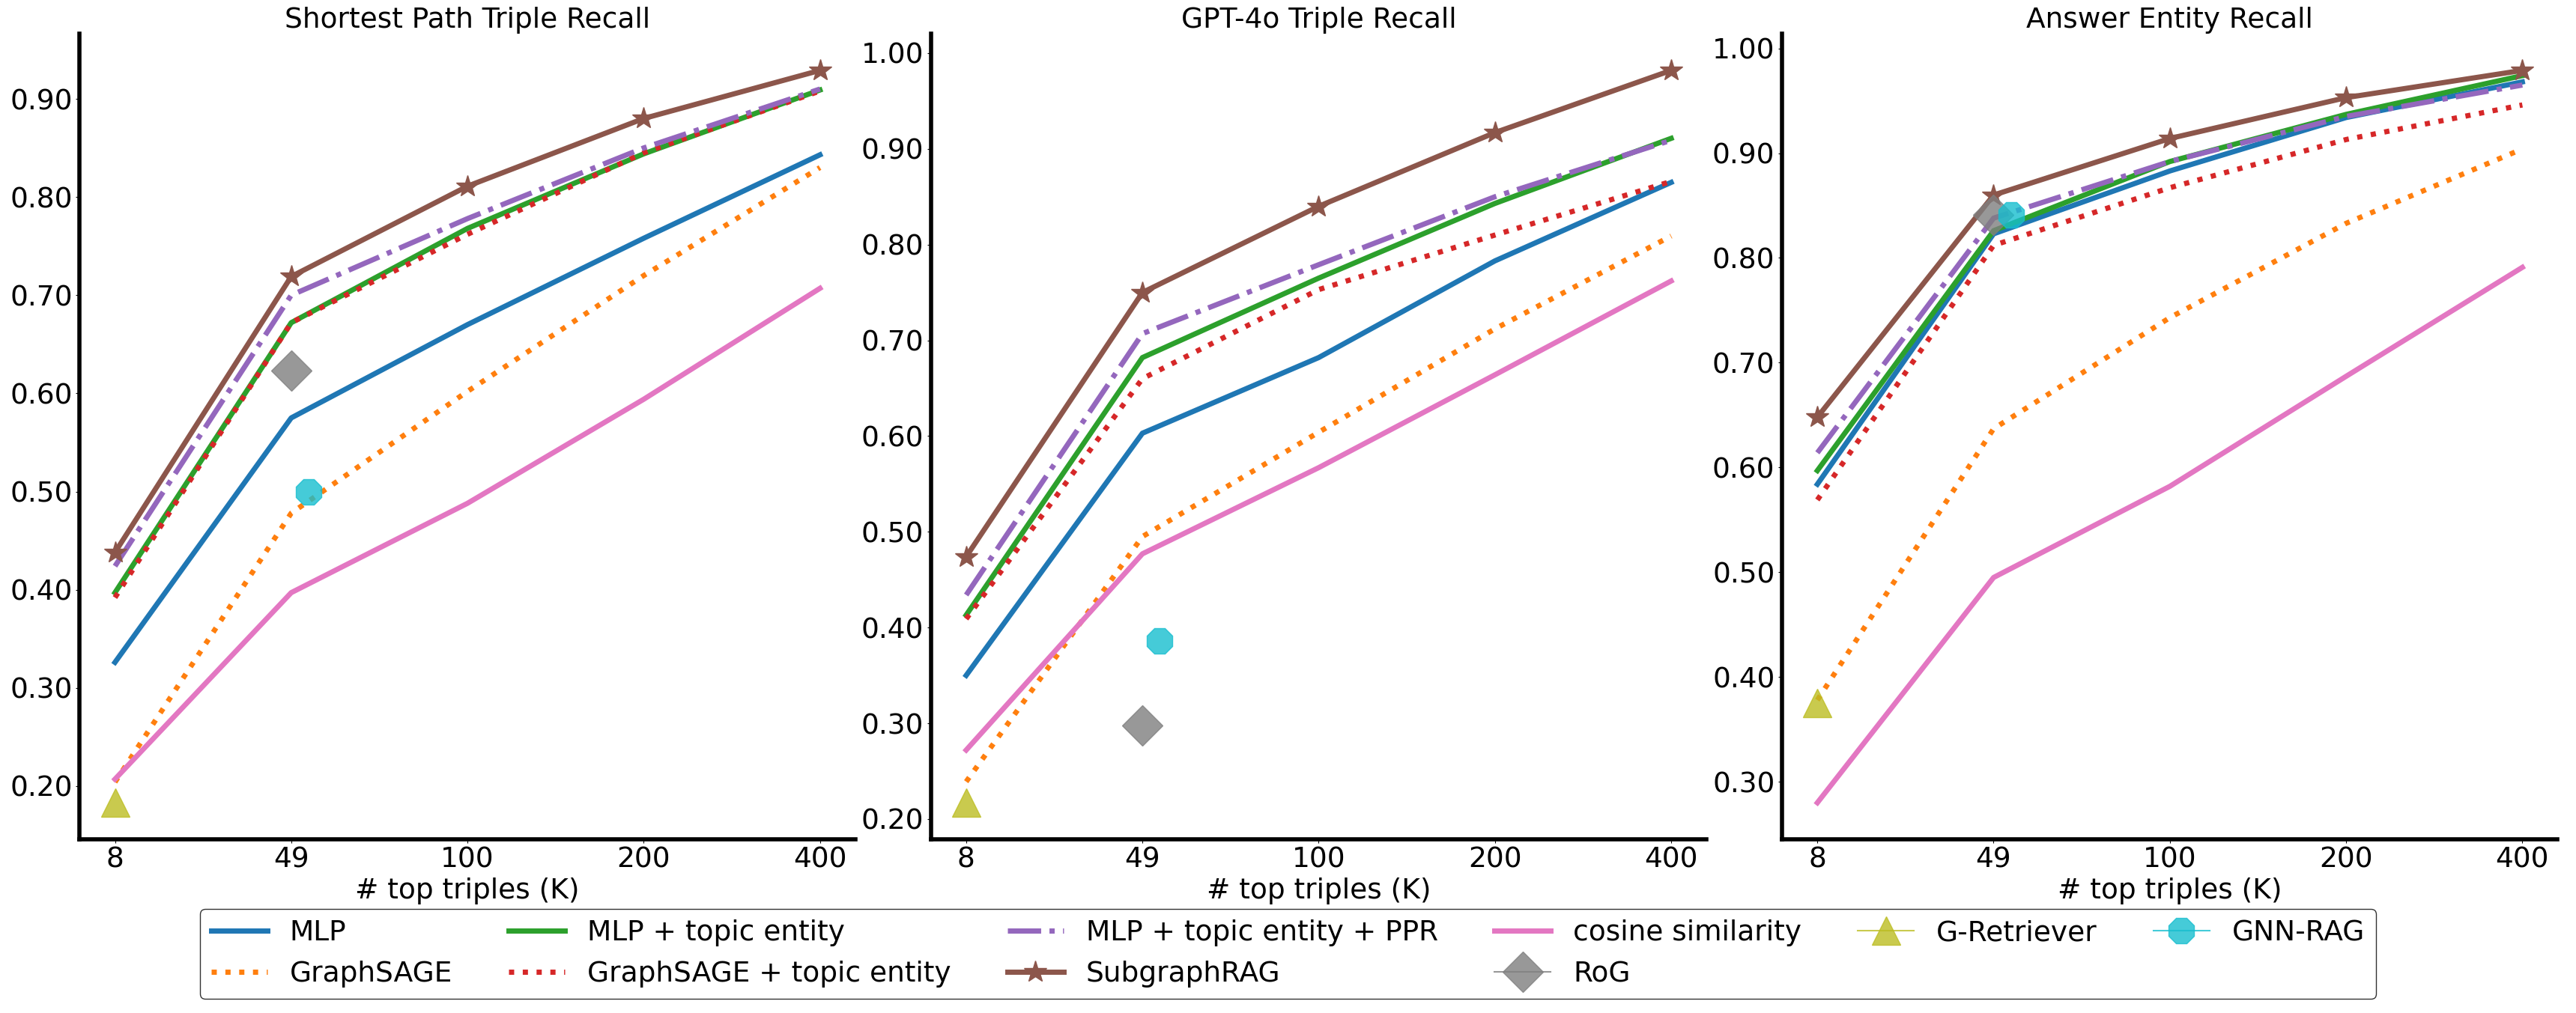
\includegraphics[trim={0.0cm 0cm 0.0cm 0cm}, clip, width=0.87\textwidth]{figs/cwq_recall_k_v6.png}
    \vspace{-3mm}
    \caption{Retrieval effectiveness on CWQ across a spectrum of $K$ values for top-$K$ triple retrieval.}
    \label{fig:cwq_k_recall}
    \vspace{-6mm}
\end{figure*}

\subsection{Evaluation for Retrieval (\textbf{Q1} \& \textbf{Q2})} 

\label{sec: retrieval_main}

\textbf{Baseline Retrievers.} 
\textbf{Cosine similarity} performs structure-free triple retrieval based on triple embeddings~\citep{li2023graph}. \textbf{SR+NSM w E2E}~\citep{zhang2022subgraph} and \textbf{Retrieve-Rewrite-Answer}~\citep{wu2023retrieve} propose constrained path search based on pre-trained text encoders. \textbf{RoG}~\citep{luo2024rog} adopts a similar strategy but fine-tunes an LLM for relation path prediction. \textbf{G-Retriever}~\citep{he2024g} combines cosine similarity search with combinatorial optimization to construct a connected subgraph. \textbf{GNN-RAG} employs lightweight GNNs to predict answer entities and extracts shortest paths between them and topic entities~\citep{mavromatis-karypis-2022-rearev, mavromatis2024gnn}.

\textbf{Implementation Details.} We adopt gte-large-en-v1.5~\citep{li2023towards} as the pre-trained text encoder for both the cosine similarity baseline and \proj, a 434M model that achieves a good balance between efficiency and English retrieval performance, as evidenced by the Massive Text Embedding Benchmark (MTEB) leaderboard~\citep{muennighoff-etal-2023-mteb}. For supervision signals, there are no ground-truth relevant subgraphs for a query $q$. Previous path-based subgraph retrievers adopt the shortest paths between the topic and answer entities for the weak supervision signals~\citep{zhang2022subgraph, luo2024rog}. We also utilize these shortest paths as the heuristic relevant subgraphs $\tilde{\gG}_q$ to train $\mathbb{Q}_{\theta}$ as in  Eq.~\ref{eq:MLE}. To reduce the size of candidate triples $\gG$, we construct subgraphs centered at topic entities $\gT_q$, following previous works. See Appendix~\ref{appendix:retrieval_exp_details} for more details.

\begin{wraptable}{r}{0.45\textwidth}  
\vspace{-0.4cm}
\caption{
Question-answering performance on WebQSP and CWQ. Best results are in \underline{\textbf{bold}}. 
By default, our reasoners use the top 100 retrieved triples. Results with 200 and 500 triples (indicated in parentheses) are also shown. Results with ($\leftrightarrow$) evaluate retriever generalizability, where the retriever is trained on one dataset and applied to the other.}
\vspace{-5mm}
\label{tab:QA_main}
\centering
\begin{adjustbox}{width=\linewidth}
\begin{tabular}{lcccc}
\\
\toprule
 & \multicolumn{2}{c}{WebQSP} & \multicolumn{2}{c}{CWQ} \\
\cmidrule(lr){2-3} \cmidrule(lr){4-5} 
      & Macro-F1     & Hit & Macro-F1 & Hit \\
\midrule
UniKGQA &
$72.2$ & 
- & 
$49.0$ &
- \\
SR+NSM w E2E & 
$64.1$
&  -
& $46.3$
& - 
\\
KD-CoT  & 52.5 & 68.6 & - & 55.7 \\
ToG (GPT-4) & - & 82.6 & - & \underline{\textbf{67.6}} \\
StructGPT & - & 74.69 & - & - \\
Retrieve-Rewrite-Answer & - &  79.36 & - & - \\
G-Retriever & 53.41 & 73.46 & - & - \\
RoG-Joint & 70.26 & 86.67 & 54.63 & 61.94 \\
RoG-Sep & 66.45 & 82.19 & 53.87 & 60.55 \\
EtD & - & $82.5$ & - & $62.0$  
\\
GNN-RAG &
$71.3$ &
$85.7$ &
$59.4$ &
$66.8$ \\
\midrule
\proj + Llama3.1-8B & 70.57 & 86.61 & 47.16 & 56.98 \\
\proj + Llama3.1-70B & 74.70 & 86.24 & 51.78 & 57.89 \\
\proj + ChatGPT & 69.21 & 83.11 & 49.13 & 56.27 \\
\proj + GPT4o-mini & 77.45 & 90.11 & 54.13 & 62.02 \\
\proj + GPT4o & 76.46 & 89.80 & 59.08 & 66.69 \\

\midrule
\proj + GPT4o-mini (200) & 77.82 & 90.54 & 54.69 & 63.49 \\
\proj + GPT4o (200) & \underline{\textbf{78.24}} & 90.91 & \underline{\textbf{59.42}} & {{67.49}} \\
\proj + GPT4o-mini (500) & 77.67 & \underline{\textbf{91.22}} & 55.41 & 64.97 \\
\midrule
\proj + Llama3.1-8B ($\leftrightarrow$) & 66.42 & 83.42 & 37.96 & 48.57 \\
\proj + GPT4o-mini ($\leftrightarrow$) & 73.81 & 88.08 & 44.69 & 54.21 \\
\proj + GPT4o-mini ($\leftrightarrow$, 500) & 76.20 & 91.22 & 50.30 & 60.80
\\

\proj + GPT4o ($\leftrightarrow$)
& 74.27 & 87.10 & 47.55 & 54.89 
\\

\proj + GPT4o ($\leftrightarrow$, 500)
& 77.12 & 89.68 & 55.14 & 62.98
\\
\bottomrule
\end{tabular}
\end{adjustbox}
\vspace{-4mm}
\end{wraptable}

\textbf{Evaluation Metrics.} Our evaluation covers both effectiveness and efficiency. For effectiveness, we employ three recall metrics, respectively for shortest path triples (i.e., $\tilde{\gG}_q$), GPT-4o-identified relevant triples, and answer entities within retrieved subgraphs. The first metric assesses the retrieval of weak supervision signals used for training. For a more accurate assessment, we employ GPT-4o to identify $\leq 20$ relevant triples for all test samples, potentially capturing relevant triples beyond the shortest paths (see Appendix~\ref{appendix:prompt} for labeling details). We calculate individual recall values per question and then take the average. For efficiency, we measure wall clock time on a 48GB NVIDIA RTX 6000 Ada GPU in seconds. To focus on model computational efficiency, we exclude KG query time. For text embedding, employed by SubgraphRAG variants and most baselines (cosine similarity, G-Retriever, and GNN-RAG), we only count the time for question embedding as the entity and relation embeddings for the entire KG can be pre-computed. Such pre-computation may yield a time-memory trade-off.

\textbf{Overall Evaluation (\textbf{Q1}).} Table~\ref{tab: main_retriever} shows that \proj consistently outperforms all other approaches in retrieval effectiveness. RoG achieves the most competitive baseline performance for retrieving shortest path triples. However, when evaluated on GPT-4o-labeled triples, RoG's performance drops significantly ($45.6\%$ for WebQSP, $52.2\%$ for CWQ), while \proj remains robust ($2.0\%$ decrease for WebQSP, $3.6\%$ increase for CWQ). This stark difference, despite using the same training signals, empirically validates that \proj's individual triple selection mechanism allows for more flexible and effective subgraph extraction compared to RoG's constrained path search approach. Regarding \textbf{efficiency}, \proj is only slightly slower than the cosine similarity baseline on WebQSP while being one to two orders of magnitude faster than other baselines, including GNN-RAG. For the cosine similarity baseline and \proj, we report recall metrics based on the top-$100$ retrieved triples ($2.3\%$ of total candidate triples on average). This budget consistently yields robust reasoning performance across LLMs in subsequent experiments. 

\textbf{Generalizability.} We further examine the generalizability of the retrievers by training them on dataset $A$ and evaluating on dataset $B$, denoted as $A\rightarrow B$ in Table~\ref{tab: main_retriever}. Despite an anticipated performance degradation, \proj consistently outperforms the alternative approaches.

\textbf{Ablation Study for Design Options and Retrieval Size.} To evaluate individual component contributions, we conduct an ablation study with several variants. $\textbf{MLP}$ is a structure-free variant employing only text embeddings. We consider \textbf{GraphSAGE}~\citep{NIPS2017_5dd9db5e}, a popular GNN, to update entity representations prior to the triple scoring. We further augment both MLP and GraphSAGE with a one-hot-encoding topic entity indicator (\textbf{MLP + topic entity} and \textbf{GraphSAGE + topic entity}). Following~\citet{sun-etal-2018-open}, we incorporate Personalized PageRank (PPR)~\citep{10.1145/511446.511513}, seeded from the topic entities, to integrate structural information (\textbf{MLP + topic entity + PPR}). To account for both the varying capabilities of downstream LLMs and inference cost/latency constraints, we evaluate these variants across a broad spectrum of retrieval sizes ($K$).

Fig.~\ref{fig:cwq_k_recall} presents the results on CWQ, with baselines included for reference. Larger retrieval sizes uniformly improve recall across all variants. Equipped with DDE, \proj outperforms other variants, even at the relatively small average retrieval sizes of the baselines. This demonstrates that \proj's superiority is not solely attributable to larger retrieval sizes. Regarding design options, the topic entity indicator invariably leads to an improvement. In contrast, GNN variants often result in performance degradation compared to their MLP counterparts. We suspect that the diffusion of semantic information introduces noise in triple selection. Finally, PPR fails to reliably yield improvements. For the results on WebQSP, see Appendix~\ref{appendix:retrieval_k}, which are also consistent.

\textbf{Multi-Hop and Multi-Topic Questions (\textbf{Q2}).} To evaluate the effectiveness of various approaches in capturing structural information for complex multi-hop and multi-topic questions, we group questions based on the number of hops and topic entities. Table~\ref{tab:retrieval_hop} presents the performance breakdown by hop count. \proj consistently outperforms other methods on WebQSP and achieves the best overall performance on CWQ. Notably, while the cosine similarity baseline and RoG demonstrate competitive performance for single-hop questions, their performance degrades significantly for multi-hop questions. Appendix~\ref{appendix:break_topic} provides a performance breakdown for single-topic and multi-topic questions, focusing exclusively on CWQ due to the predominance of single-topic questions in the WebQSP test set ($98.3\%$). \proj consistently exhibits superior performance across all metrics for both single-topic and multi-topic questions. Our comprehensive analysis highlights the remarkable effectiveness of DDE in capturing complex topic-centered structural information essential for challenging questions involving multi-hop reasoning and multiple topic entities.

\subsection{KGQA Results (\textbf{Q3} \& \textbf{Q4})}
\label{sec:kgqa}

\textbf{KGQA Baselines.} Besides the baselines in retrieval evaluation, we include more KGQA methods, including UniKGQA~\citep{jiang2023unikgqa}, KD-CoT~\citep{wang2023knowledge}, StructGPT~\citep{jiang2023structgpt}, ToG~\citep{sun2024think}, and EtD~\citep{liu2024explore}. 
For RoG, we present two entries: RoG-Joint and RoG-Sep. Originally, RoG fine-tuned its LLMs on the training sets of both WebQSP and CWQ. Yet, this joint training approach leads to significant label leakage, with over 50\% of WebQSP test questions (or their variants) appearing in CWQ's training set, and vice versa. Therefore, we re-trained RoG on each dataset separately, denoted by RoG-Sep.

\textbf{Evaluation Metrics.} 
Along with the commonly reported Macro-F1 and Hit\tablefootnote{The baselines claim to report Hit@1, but they actually compute Hit, which measures whether at least one correct answer appears in the LLM response.}, we also include Micro-F1 to account for the imbalance in the number of ground-truth answers across samples and Hit@1 for a more inclusive evaluation. To further assess model performance, we introduce score$_h$, inspired by~\citep{yang2024crag}, which evaluates how truth-grounded the predicted answers are and the degree of hallucination. This metric penalizes hallucinated answers while favoring missing answers over incorrect ones. Scores are normalized to a range of 0 to 100, with higher scores indicating better truth-grounding in the model’s answers. The scoring strategy is described in detail in Appendix~\ref{appx:score}.

\vspace{-3mm}
\begin{table}[t]
\caption{
Question-answering performance on WebQSP-sub and CWQ-sub. Best results are in \underline{\textbf{bold}}. 
By default, our reasoners use the top 100 retrieved triples. Results with 200 and 500 triples (indicated in parentheses) are also shown. Results with ($\leftrightarrow$) evaluate retriever generalizability, where the retriever is trained on one dataset and applied to the other.}
\vspace{-4mm}
\label{tab:QA_sub}
\centering
\begin{adjustbox}{width=0.8\textwidth}
\begin{tabular}{lcccccccccc}
\\
\toprule
 & \multicolumn{5}{c}{WebQSP-sub} & \multicolumn{5}{c}{CWQ-sub} \\
\cmidrule(lr){2-6} \cmidrule(lr){7-11}
      & Macro-F1 & Micro-F1 & Hit & Hit@1 & Score$_{h}$ & Macro-F1 & Micro-F1 & Hit & Hit@1 & Score$_{h}$\\
\midrule 
SR+NSM w E2E & 58.79 & 37.04 & 68.63 & 60.62 & 64.44 & - & - & - & - & - 
\\
G-Retriever & 54.13 & 23.84 & 74.52 & 67.56 & 67.97 & - & - & - & - & - \\
RoG-Joint & 72.01 & 47.70 & 88.90 & 82.62 & 76.13 & 58.61 & 52.12 & 66.22 & 61.17 & 55.15 \\
RoG-Sep & 67.94 & 43.10 & 84.03 & 77.61 & 72.79 & 57.69 & 52.83 & 64.64 & 60.64 & 54.51 \\
\midrule
\proj + Llama3.1-8B & 72.10 & 46.56 & 88.58 & 84.80 & 82.42 & 54.76 & 51.76 & 65.80 & 59.69 & 62.89 \\
\proj + Llama3.1-70B & 75.97 & 51.64 & 87.88 & 85.89 & \underline{\textbf{85.57}} & 61.49 & 59.91 & 68.43 & 65.52 & \underline{\textbf{67.62}} \\
\proj + ChatGPT & 70.81 & 44.73 & 85.18 & 80.82 & 81.53 & 56.37 & 54.44 & 64.40 & 60.99 & 61.31 \\
\proj + GPT4o-mini & 78.34 & 58.44 & 91.34 & 87.36 & 82.21 & 61.13 & 58.86 & 70.01 & 65.48 & 64.20 \\
\proj + GPT4o & 77.61 & 56.78 & 91.40 & 86.40 & 81.85 & 65.99 & \underline{\textbf{63.18}} & 73.91 & 68.89 & 66.57 \\
\midrule

\proj + GPT4o-mini (200) & 78.66 & 58.65 & 91.73 & 87.04 & 81.98 & 61.58 & 57.47 & 71.45 &  65.87 & 63.66 \\
\proj + GPT4o (200) & \underline{\textbf{79.40}} & \underline{\textbf{58.91}} & \underline{\textbf{92.43}} & 87.75 & 82.46 & \underline{\textbf{66.48}} & 61.30 & \underline{\textbf{75.14}} & \underline{\textbf{69.42}} & 66.45 \\
\proj + GPT4o-mini (500) & 78.46 & 57.08 & \underline{\textbf{92.43}} & \underline{\textbf{88.01}} & 81.95 & 62.18 & 56.86 & 72.82 & 66.57 & 62.77 
\\
\midrule
\proj + Llama3.1-8B ($\leftrightarrow$) & 67.91 & 42.79 & 85.25 & 81.21 & 80.09 & 43.03 & 40.73 & 55.09 & 47.58 & 56.78 \\
\proj + GPT4o-mini ($\leftrightarrow$) & 74.42 & 49.41 & 89.10 & 84.67 & 81.35 & 49.47 & 45.16 & 60.18 & 54.18 & 58.86 \\
\proj + GPT4o-mini ($\leftrightarrow$, 500)
& 76.83 & 52.01 & 92.30 & 87.43 & 81.41 & 55.58 & 49.13 & 67.24 & 59.69 & 59.87\\

\proj + GPT4o ($\leftrightarrow$)
& 74.98 & 50.67 & 88.26 & 84.73 & 83.24 & 52.40 & 52.28 & 60.36 & 56.39 & 63.70
\\

\proj + GPT4o ($\leftrightarrow$, 500)
& 77.96 & 56.40 & 90.96 & 86.66 & 83.35 & 61.96 & 58.48 & 70.47 & 64.96 & 66.86
\\

\bottomrule
\end{tabular}
\end{adjustbox}
\vspace{-3mm}
\end{table}

\begin{table}[t]
\caption{Breakdown of QA performance by reasoning hops.}
\vspace{-3mm}
\label{tab:acc_hop}
\centering
\begin{adjustbox}{width=0.75\textwidth}
\begin{tabular}{lcccccccccc}
\\
\toprule
 & \multicolumn{4}{c}{WebQSP-sub} & \multicolumn{6}{c}{CWQ-sub}\\
        \cmidrule(lr){2-5} \cmidrule{6-11}
      & \multicolumn{2}{c}{$1$}  
      & \multicolumn{2}{c}{$2$}  
      & \multicolumn{2}{c}{$1$}  
      & \multicolumn{2}{c}{$2$} 
      & \multicolumn{2}{c}{$\geq 3$}  \\
      & \multicolumn{2}{c}{$(65.8 \%)$}  
      & \multicolumn{2}{c}{$(34.2 \%)$} 
      & \multicolumn{2}{c}{$(28.0 \%)$}  
      & \multicolumn{2}{c}{$(65.9 \%)$}  
      & \multicolumn{2}{c}{$(6.1 \%)$}  \\
      \cmidrule(lr){2-3} \cmidrule(lr){4-5} \cmidrule{6-7} \cmidrule{8-9} \cmidrule{10-11} 
      & Marco-F1 & Hit & Marco-F1 & Hit & Marco-F1 & Hit & Marco-F1 & Hit & Marco-F1 & Hit
\\
\midrule
G-Retriever 
& 56.41 & 78.20 & 45.73 & 65.35 & - & - & - & - & - & -
\\

RoG-Joint
& 77.05 & 92.96 & 62.53 & 81.54 & 59.75 & 66.33 & 59.70 & 68.56 & 41.46 & 43.27
\\

RoG-Sep 
& 74.50 & 89.83 & 55.62 & 73.45 & 59.35 & 66.20 & 59.45 & 67.17 & 31.33 & 33.33
\\
\midrule
\proj (Llama3.1-8B)
& 75.50 & 91.40 & 65.87 & 83.62 & 51.54 & 63.05 & 57.52 & 68.93 & 41.88 & 47.37
\\

\proj (GPT4o-mini)
& 80.56 & 92.86 & 74.11 & 88.51 & 57.36 & 67.34 & 63.85 & 72.74 & 51.14 & 54.39

\\
\bottomrule
\end{tabular}
\end{adjustbox}
\vspace{-2mm}
\end{table}

\begin{table}[t]
\caption{Ablation studies with different retrievers, using the same prompt and Llama3.1-8B-Instruct as the reasoner. Rand refers to random triple sampling, RandNoAns removes triples with ground-truth answers after random sampling, and NoRetriever directly asks questions without KG info.}
\vspace{-4mm}
\label{tab:ablation_retriever_llama3}
\centering
\begin{adjustbox}{width=\textwidth}
\begin{tabular}{rcccccccccccccc}
\\
\toprule
 & \multicolumn{2}{c}{WebQSP} & \multicolumn{2}{c}{CWQ} & \multicolumn{5}{c}{WebQSP-sub} & \multicolumn{5}{c}{CWQ-sub} \\
\cmidrule(lr){2-3} \cmidrule(lr){4-5}  \cmidrule(lr){6-10} \cmidrule(lr){11-15}
      & Macro-F1     & Hit & Macro-F1 & Hit & Macro-F1 & Micro-F1 & Hit & Hit@1 & Score$_{h}$ & Macro-F1 & Micro-F1 & Hit & Hit@1 & Score$_{h}$\\
\midrule
Rand + \proj Reasoner 
& 37.69 & 60.14 & 27.34 & 35.85 & 37.79 & 17.79 & 60.74 & 54.97 & 65.06 & 29.97 & 29.15 & 39.15 & 35.11 & 52.45
\\


RandNoAns + \proj Reasoner
& 21.18 & 33.54 & 16.40 & 22.71 & 20.61 &  8.64 & 33.03 & 27.33 & 47.29 & 16.47 & 16.44 & 23.00 & 19.42 & 43.79
\\


NoRetriever + \proj Reasoner 
& 35.86 & 51.90 & 25.64 & 32.34 & 35.03 & 17.01 & 51.38 & 47.59 & 55.57 & 27.42 & 22.66 & 33.95 & 30.65 & 44.87
\\
\midrule


cosine similarity + \proj Reasoner
& 58.41 & 74.14 & 34.59 & 43.61 & 59.26 & 37.31 & 75.43 & 71.20 & 73.16 & 39.05 & 35.48 & 49.02 & 43.68 & 55.72\\ 

Retrieve-Rewrite-Answer + \proj Reasoner 
&  8.96 & 11.43 & - & - & 9.11 & 5.23 & 11.43 & 10.84 & 63.45 & - & - & - & - & -
\\ 

StructGPT + \proj Reasoner
& 62.14 & 75.00 & - & - & 62.55& 44.72 & 75.69 & 73.57 & 80.82 & - & - & - & - & - \\

G-Retriever + \proj Reasoner
& 48.91 & 64.50 & 28.47 & 34.58 & 49.92 & 28.08 & 65.88 & 62.60 & 72.54 & 31.55 & 32.22 & 38.17 & 35.22 & 58.22
\\ 

RoG-Sep + \proj Reasoner 
& 57.68 & 74.39 & 36.85 & 45.23 & 59.36 & 40.32 & 76.65 & 72.61 & 79.69 & 44.11 & 43.69 & 54.04 & 47.68 & 66.18\\

GNN-RAG + \proj Reasoner 
& 62.34 & 78.81 & 46.40 & 54.35 & 63.93 & 42.43 & 80.89 & 77.10 & 82.86 & 55.08 & 53.38 & 64.33 & 59.76 & 67.55
\\

GNN-RAG ($\leftrightarrow$) + \proj Reasoner 
& 52.07 & 71.38 & 34.88 & 43.13 & 53.01 & 34.58 & 72.93 & 67.99 & 73.37 & 39.98 & 34.60 & 49.54 & 44.91 & 57.42
\\



\midrule
\proj 
& 70.57 & 86.61 & 47.16 & 56.98 & 72.10 & 46.56 & 88.58 & 84.80 & 82.42 & 54.76 & 51.76 & 65.80 & 59.69 & 62.89
\\

\proj ($\leftrightarrow$) & 66.42 & 83.42 & 37.96 & 48.57 & 67.91 & 42.79 & 85.25 & 81.21 & 80.09 & 43.03 & 40.73 & 55.09 & 47.58 & 56.78 
\\


\bottomrule
\end{tabular}
\end{adjustbox}
\vspace{-6mm}
\end{table}

\begin{figure*}[t]
    \vspace{-4mm}
    \centering
    \begin{subfigure}[t]{0.48\linewidth} 
        \centering
        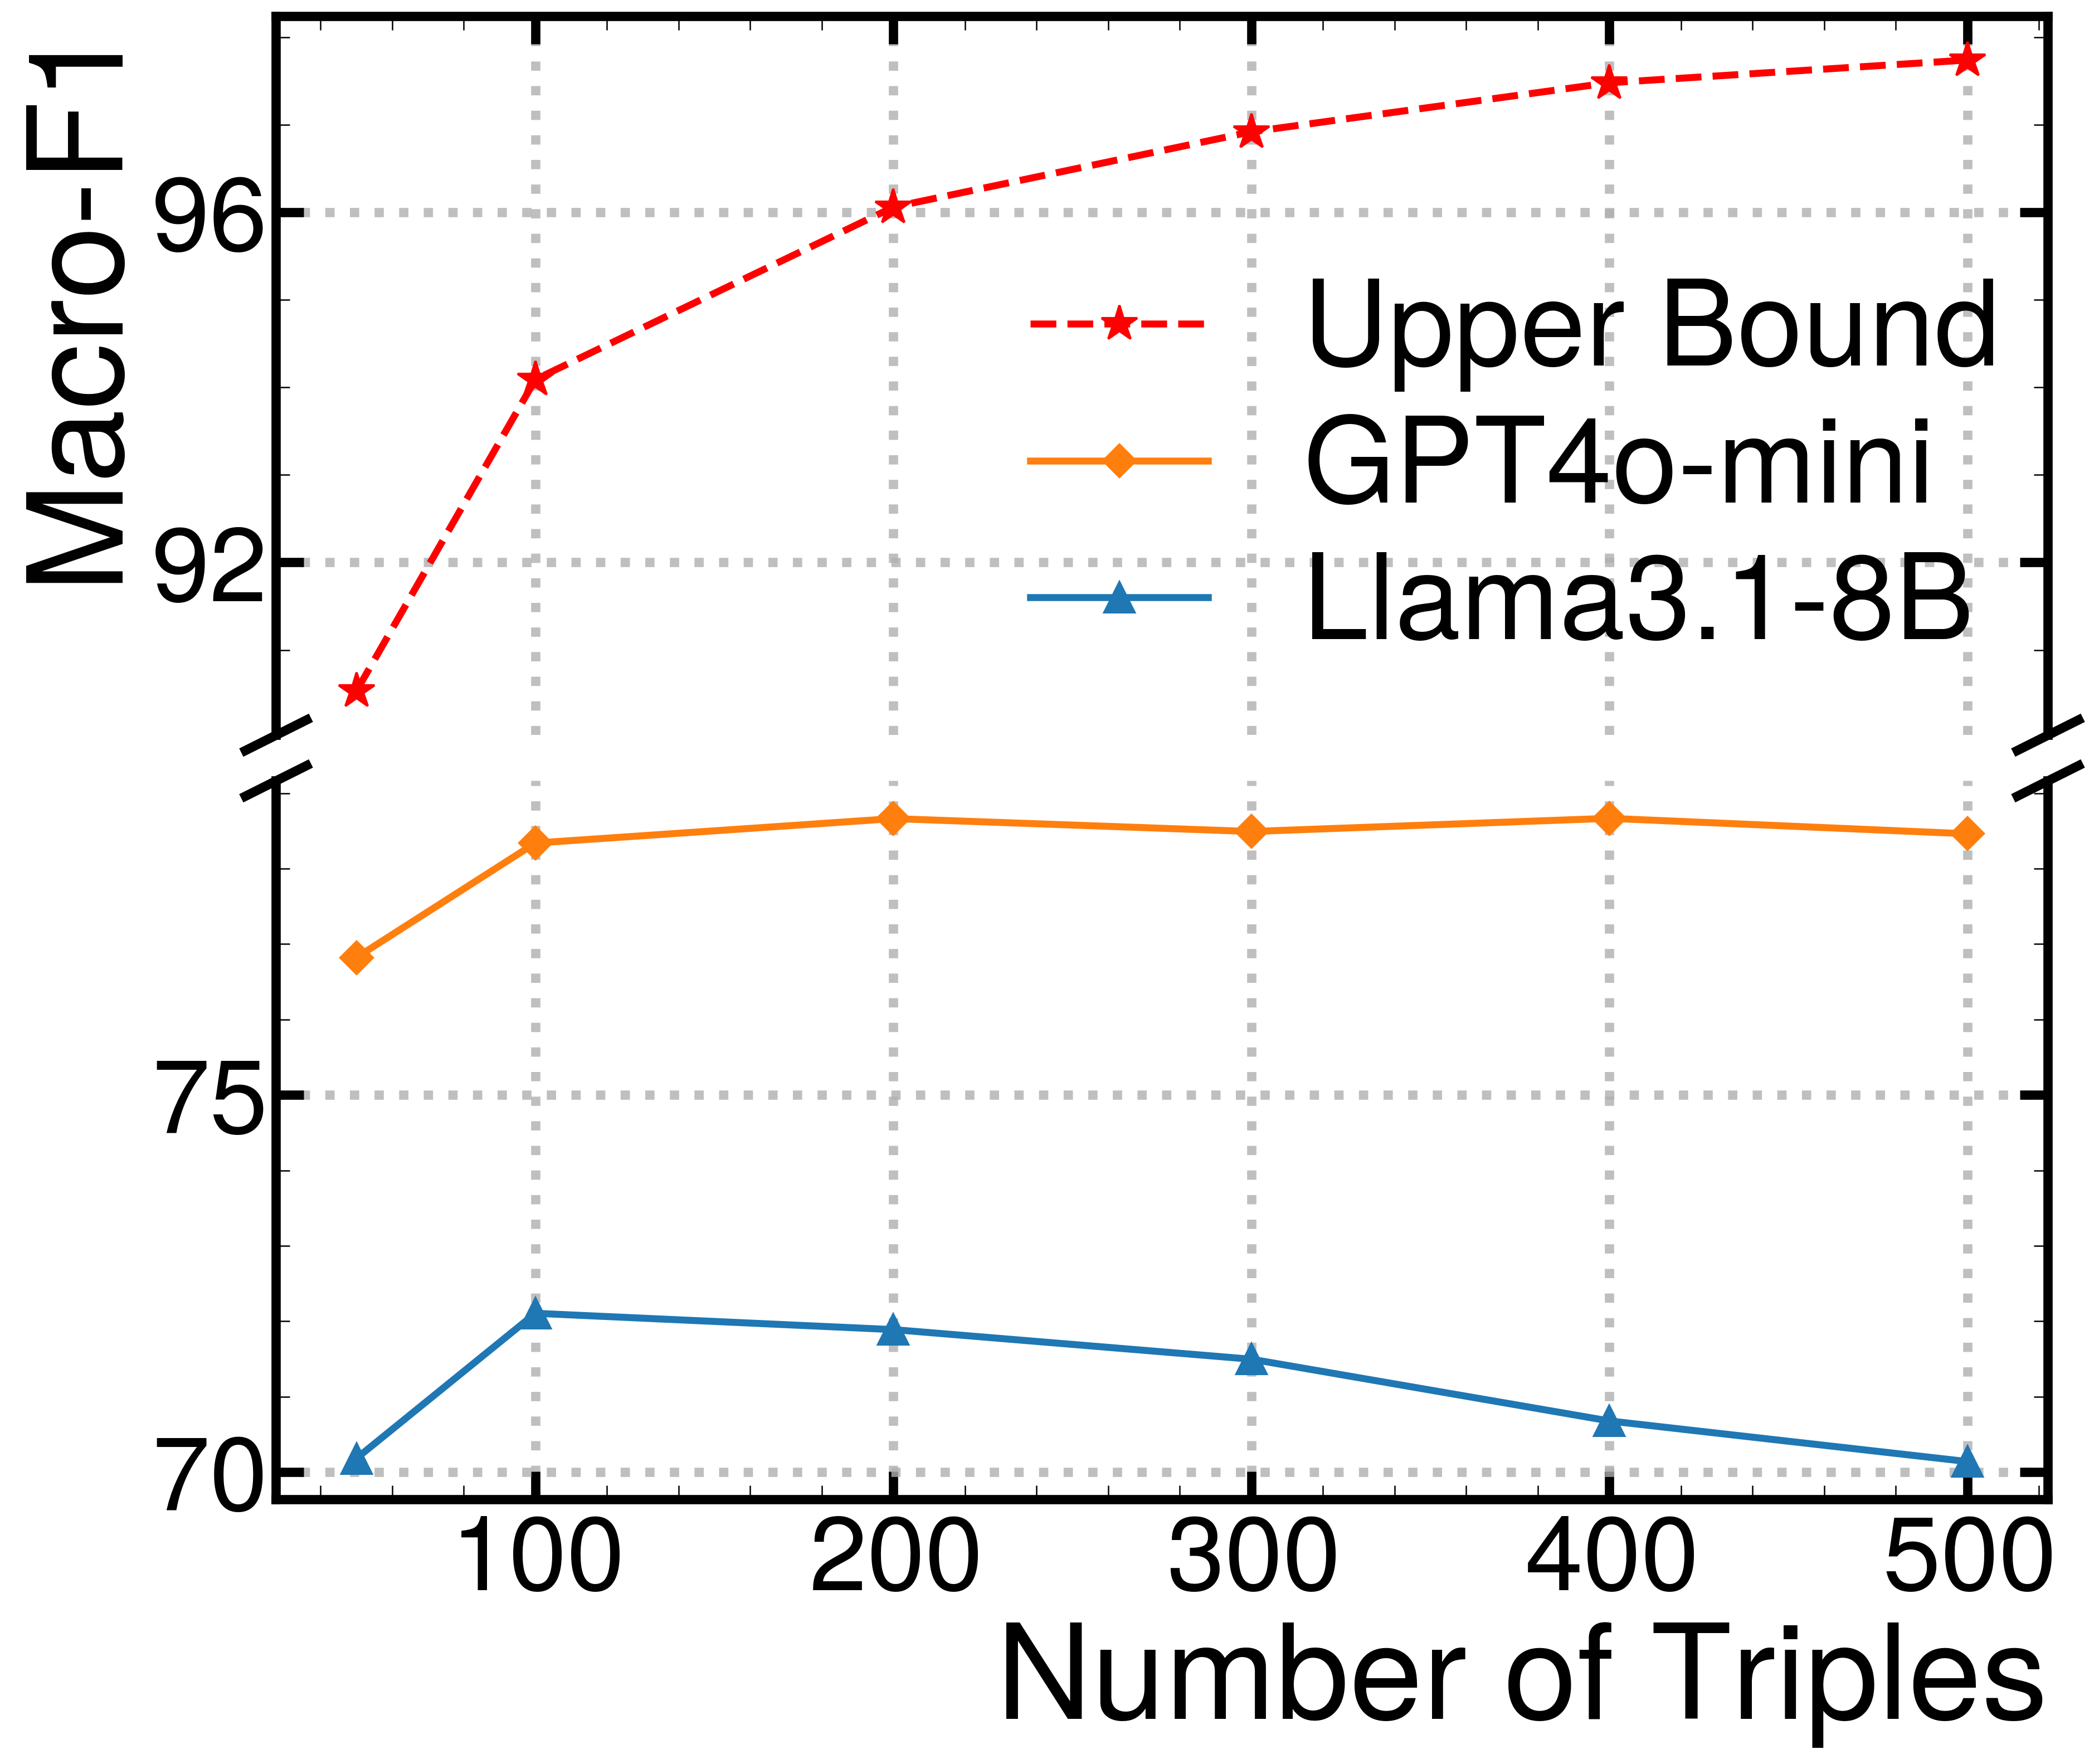
\includegraphics[trim={0cm 0.0cm 0cm 0.0cm}, clip, width=0.493\textwidth]{figs/webqsp_f1.png}
        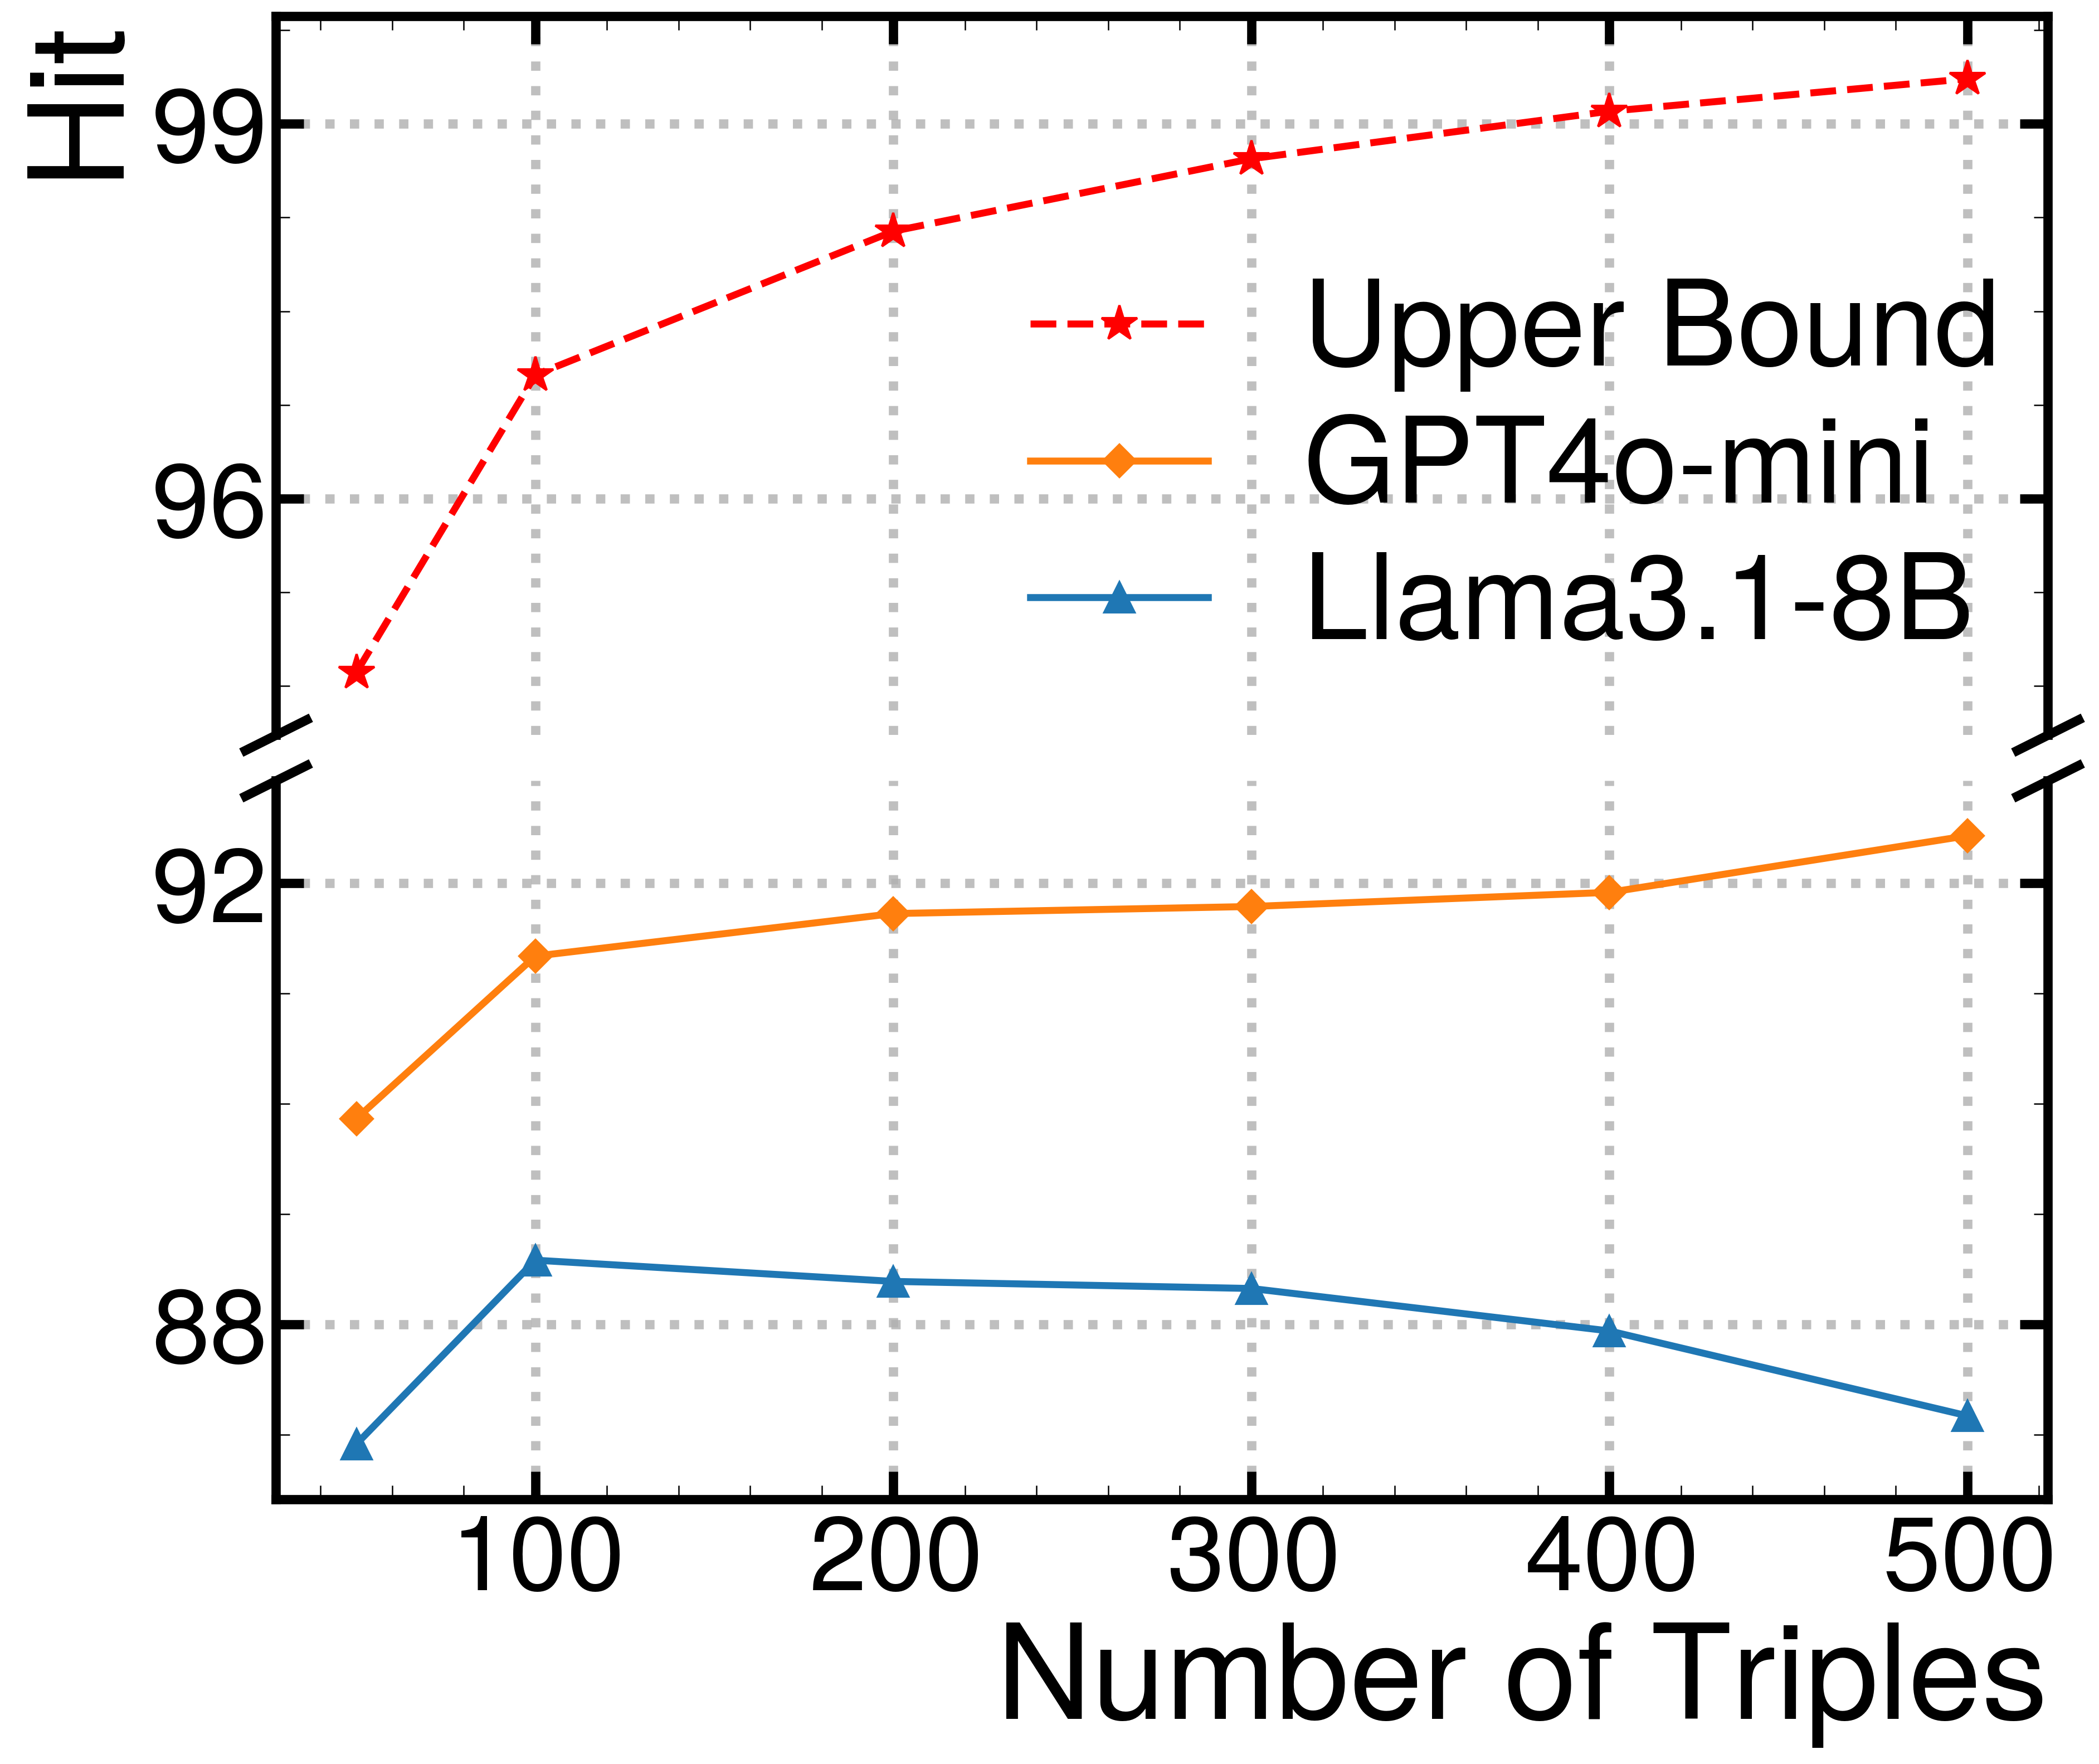
\includegraphics[trim={0cm 0.0cm 0cm 0.0cm}, clip, width=0.493\textwidth]{figs/webqsp_hit.png}
        \caption{WebQSP-sub}
    \end{subfigure}
    \hspace{0.01\linewidth}
    \begin{subfigure}[t]{0.48\linewidth}
        \centering
        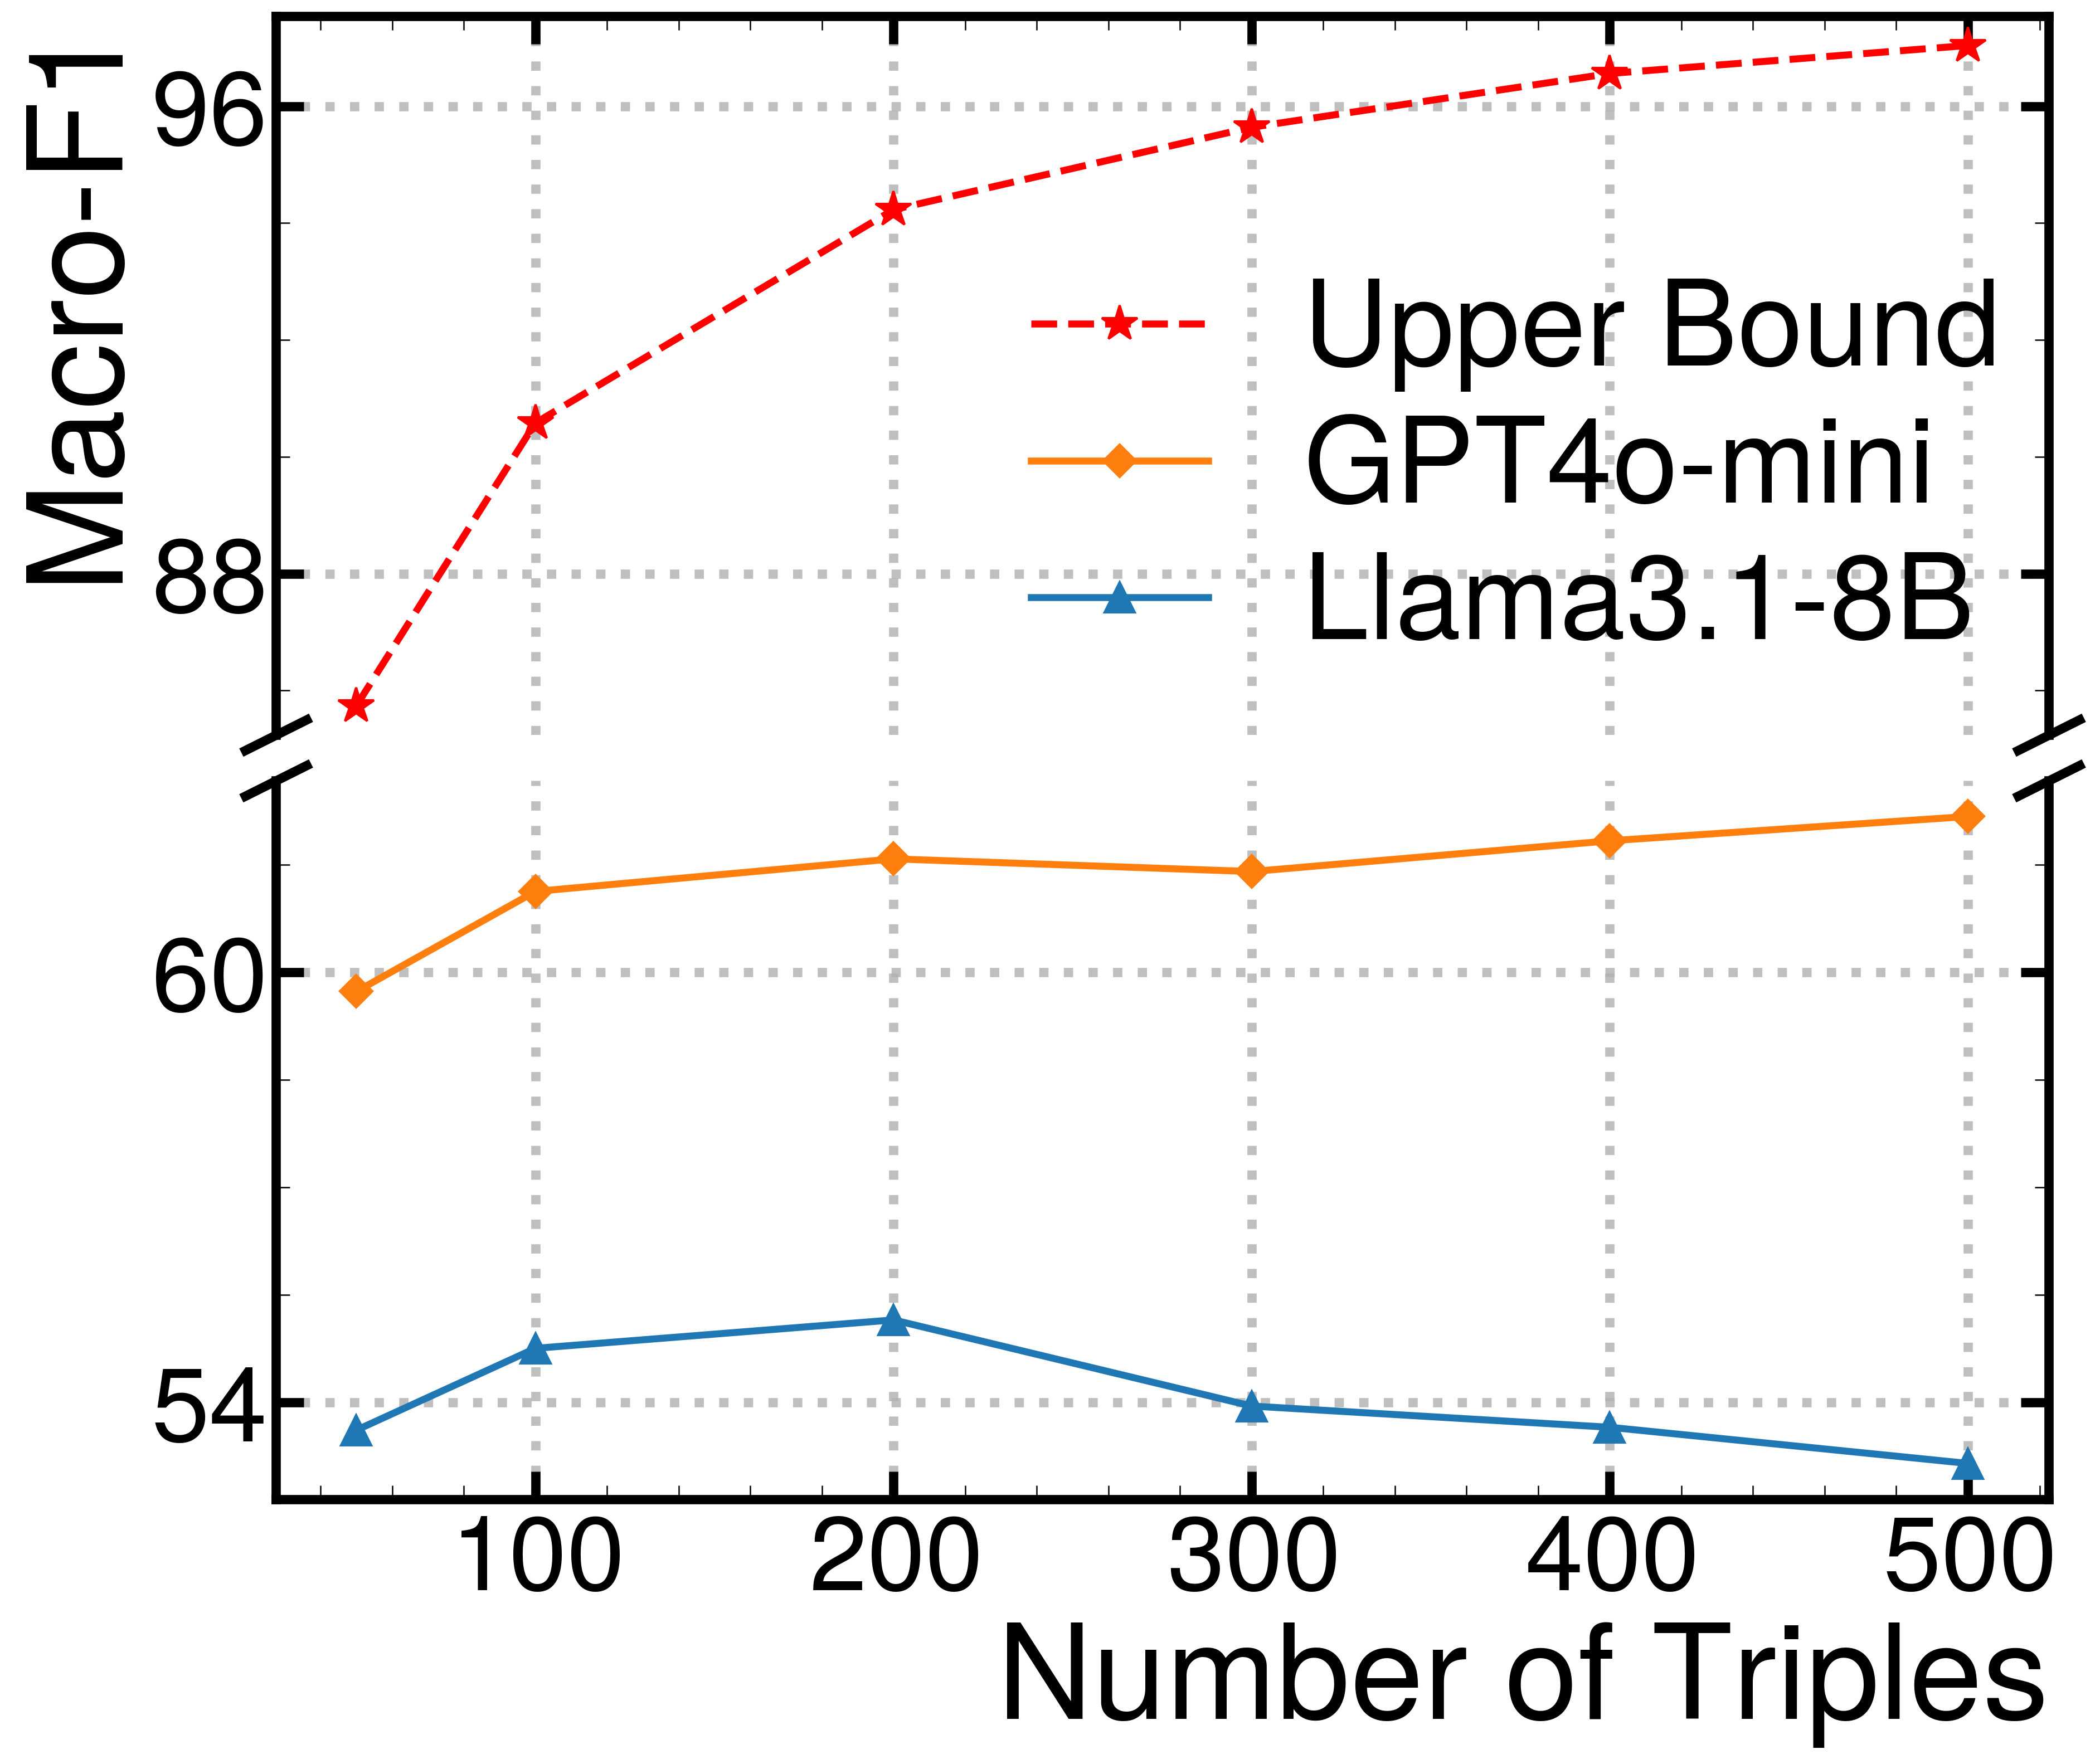
\includegraphics[trim={0cm 0.0cm 0.0cm 0cm}, clip,width=0.493\linewidth]{figs/cwq_f1.png}
        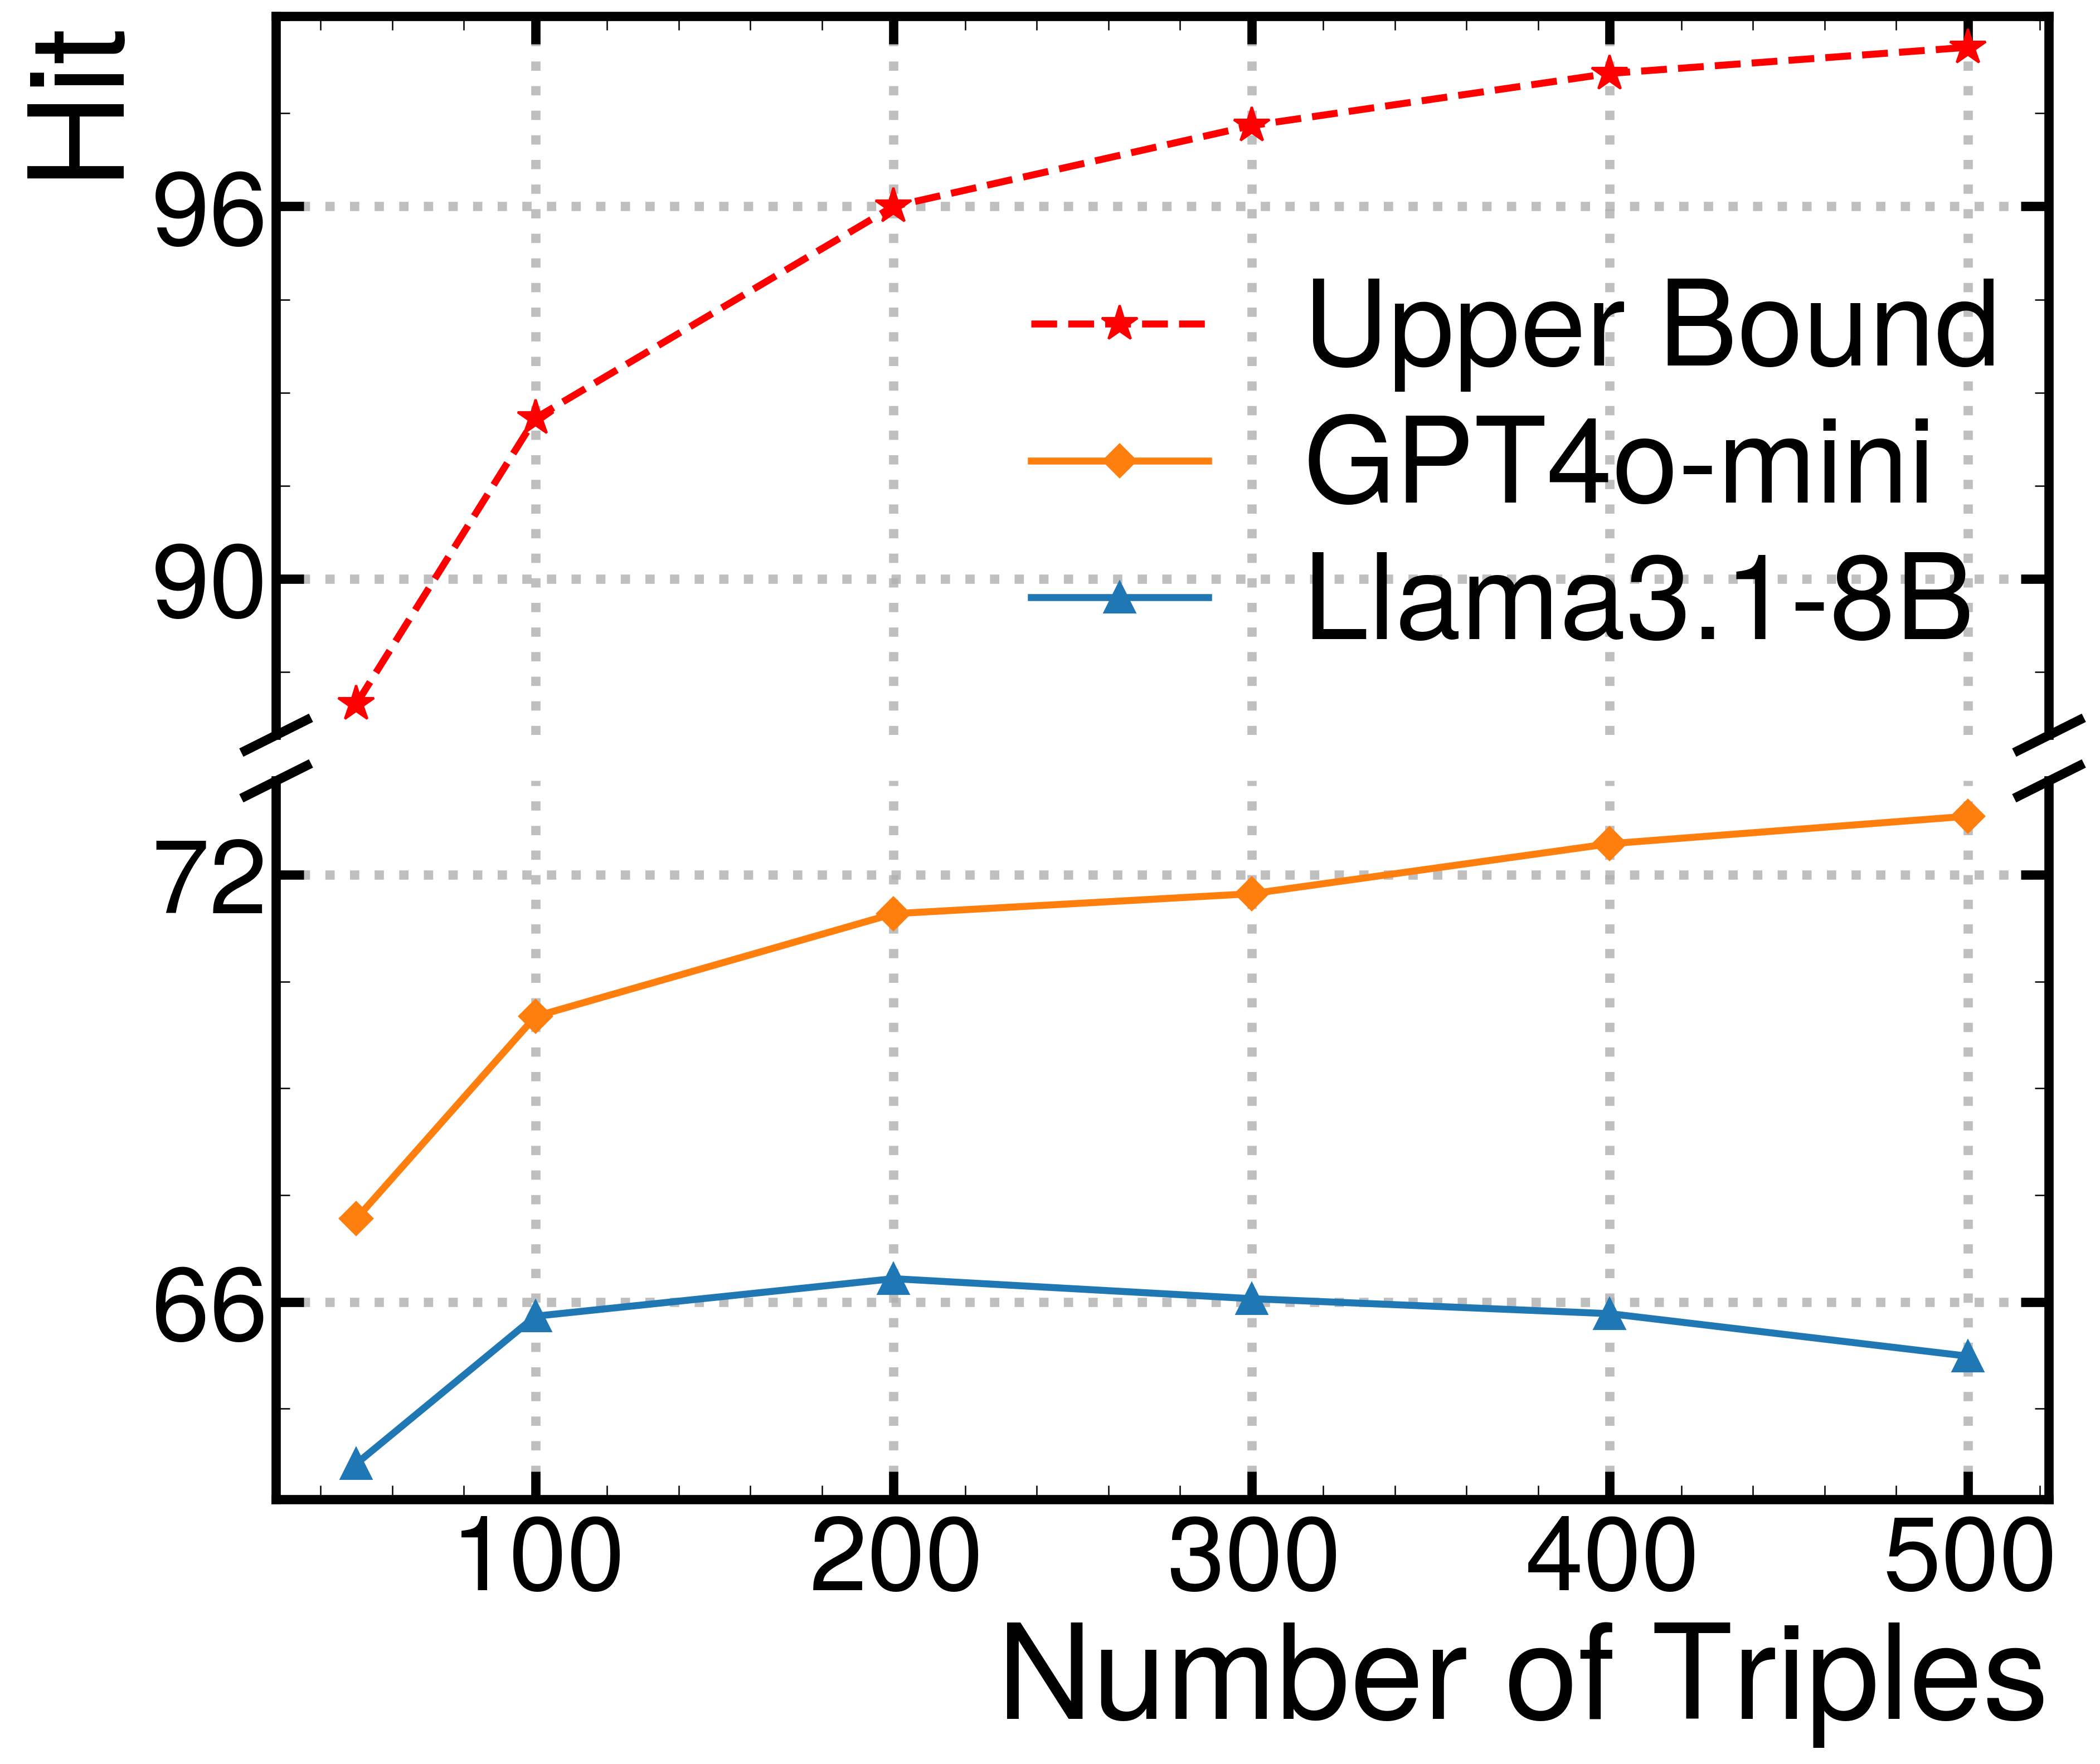
\includegraphics[trim={0cm 0.0cm 0.0cm 0cm}, clip,width=0.493\linewidth]{figs/cwq_hit.png}
        \caption{CWQ-sub}
    \end{subfigure}
    \vspace*{-2mm}
    \caption{Ablation studies on the number of retrieved triples used in LLM reasoners.}
    \label{fig:ablation_number}
    \vspace{-7mm}
\end{figure*}

% \begin{figure*}[t]
%     \vspace{-2mm}
%     \centering
%     \begin{subfigure}[t]{0.48\linewidth} 
%         \centering
%         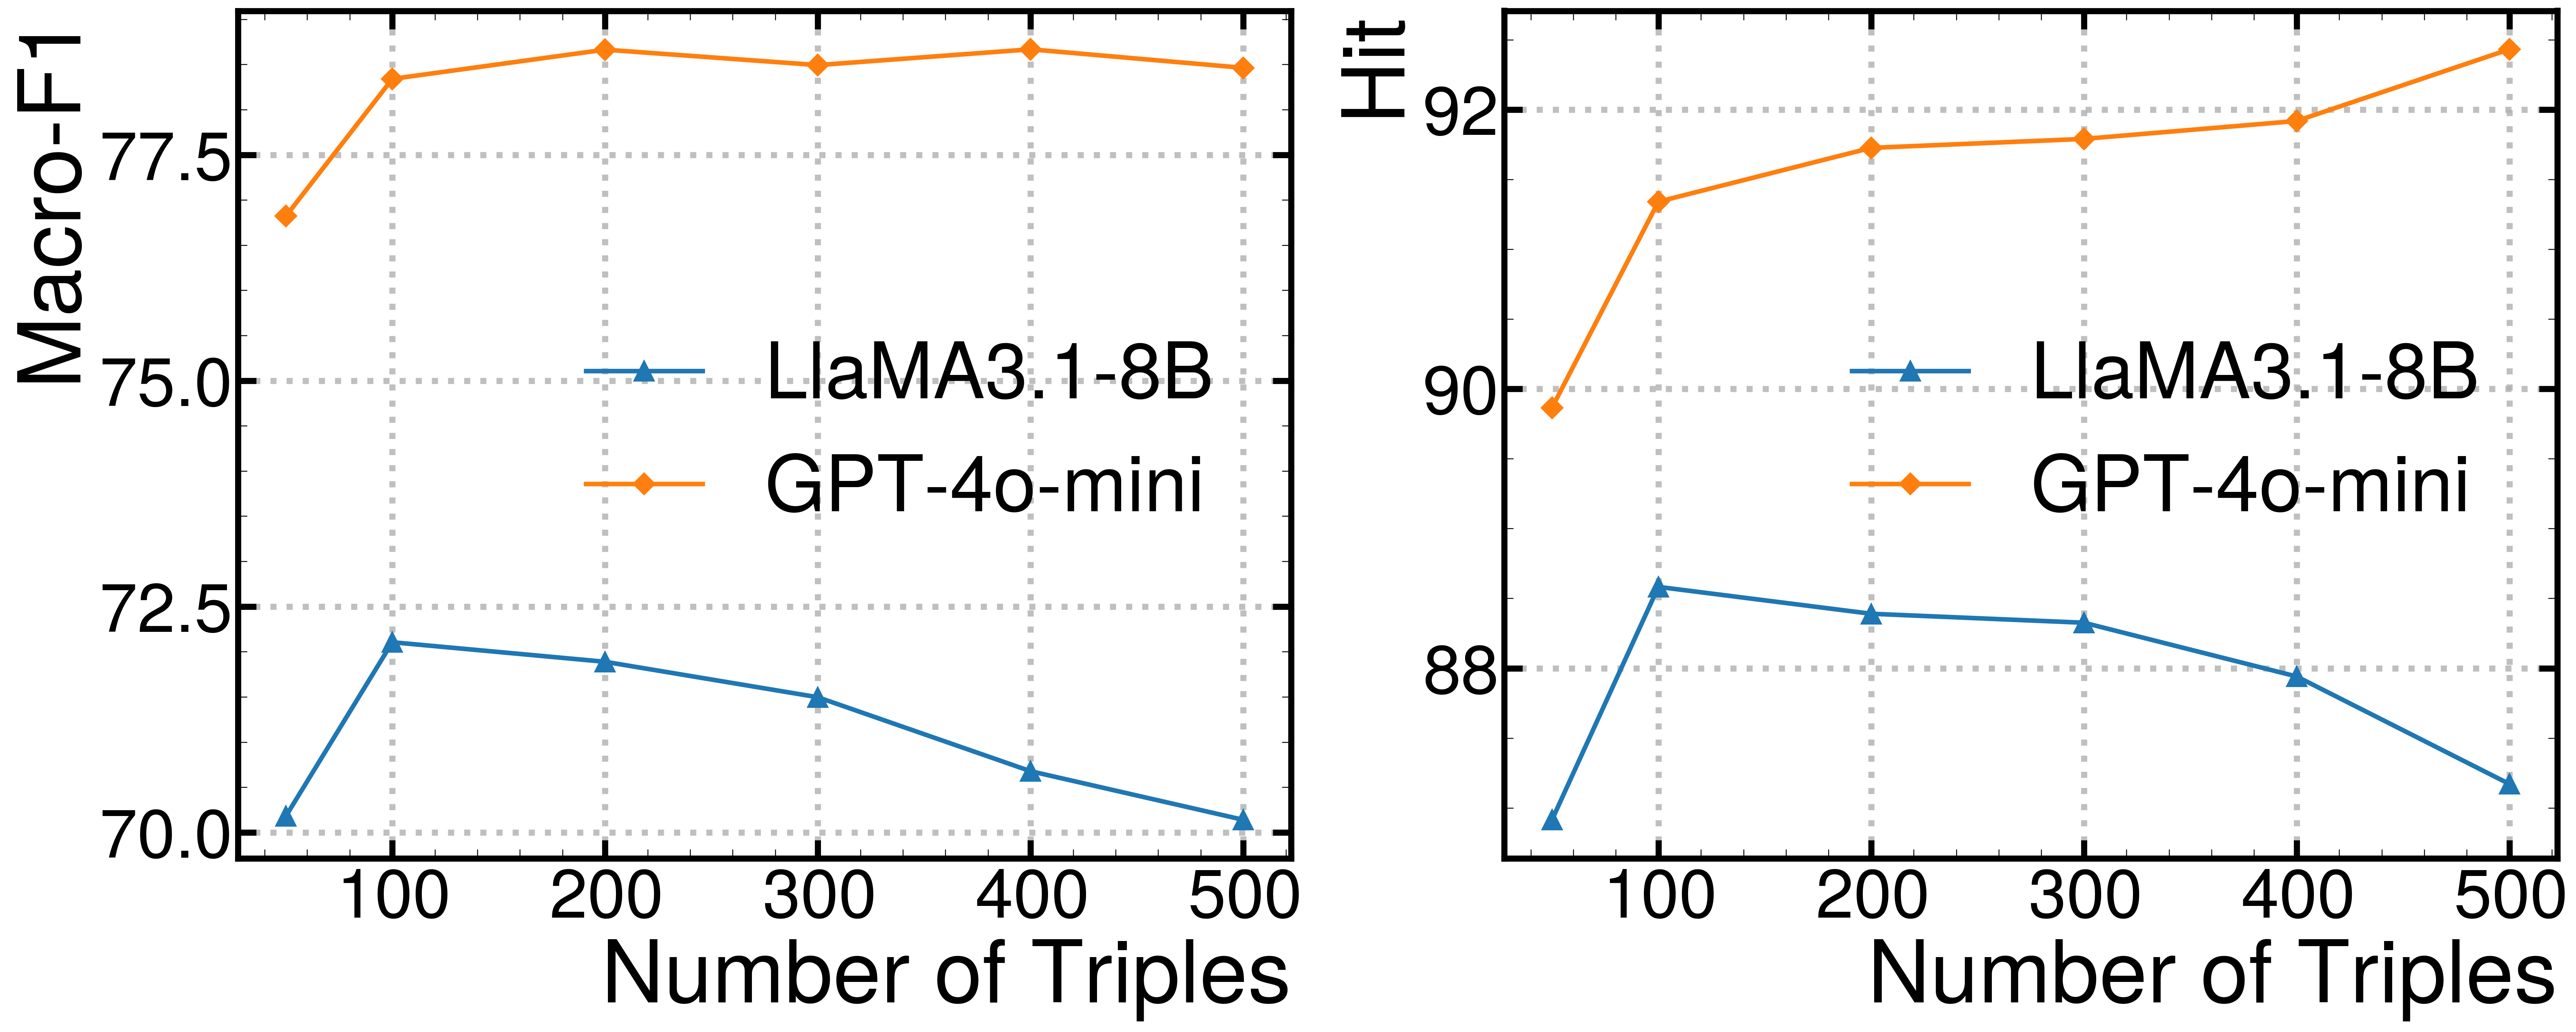
\includegraphics[trim={0cm 0.0cm 0cm 0.0cm}, clip, width=1.0\textwidth]{figs/numbers_webqsp.png}
%         \caption{WebQSP-sub}
%     \end{subfigure}
%     \hspace{0.01\linewidth}
%     \begin{subfigure}[t]{0.48\linewidth}
%         \centering
%         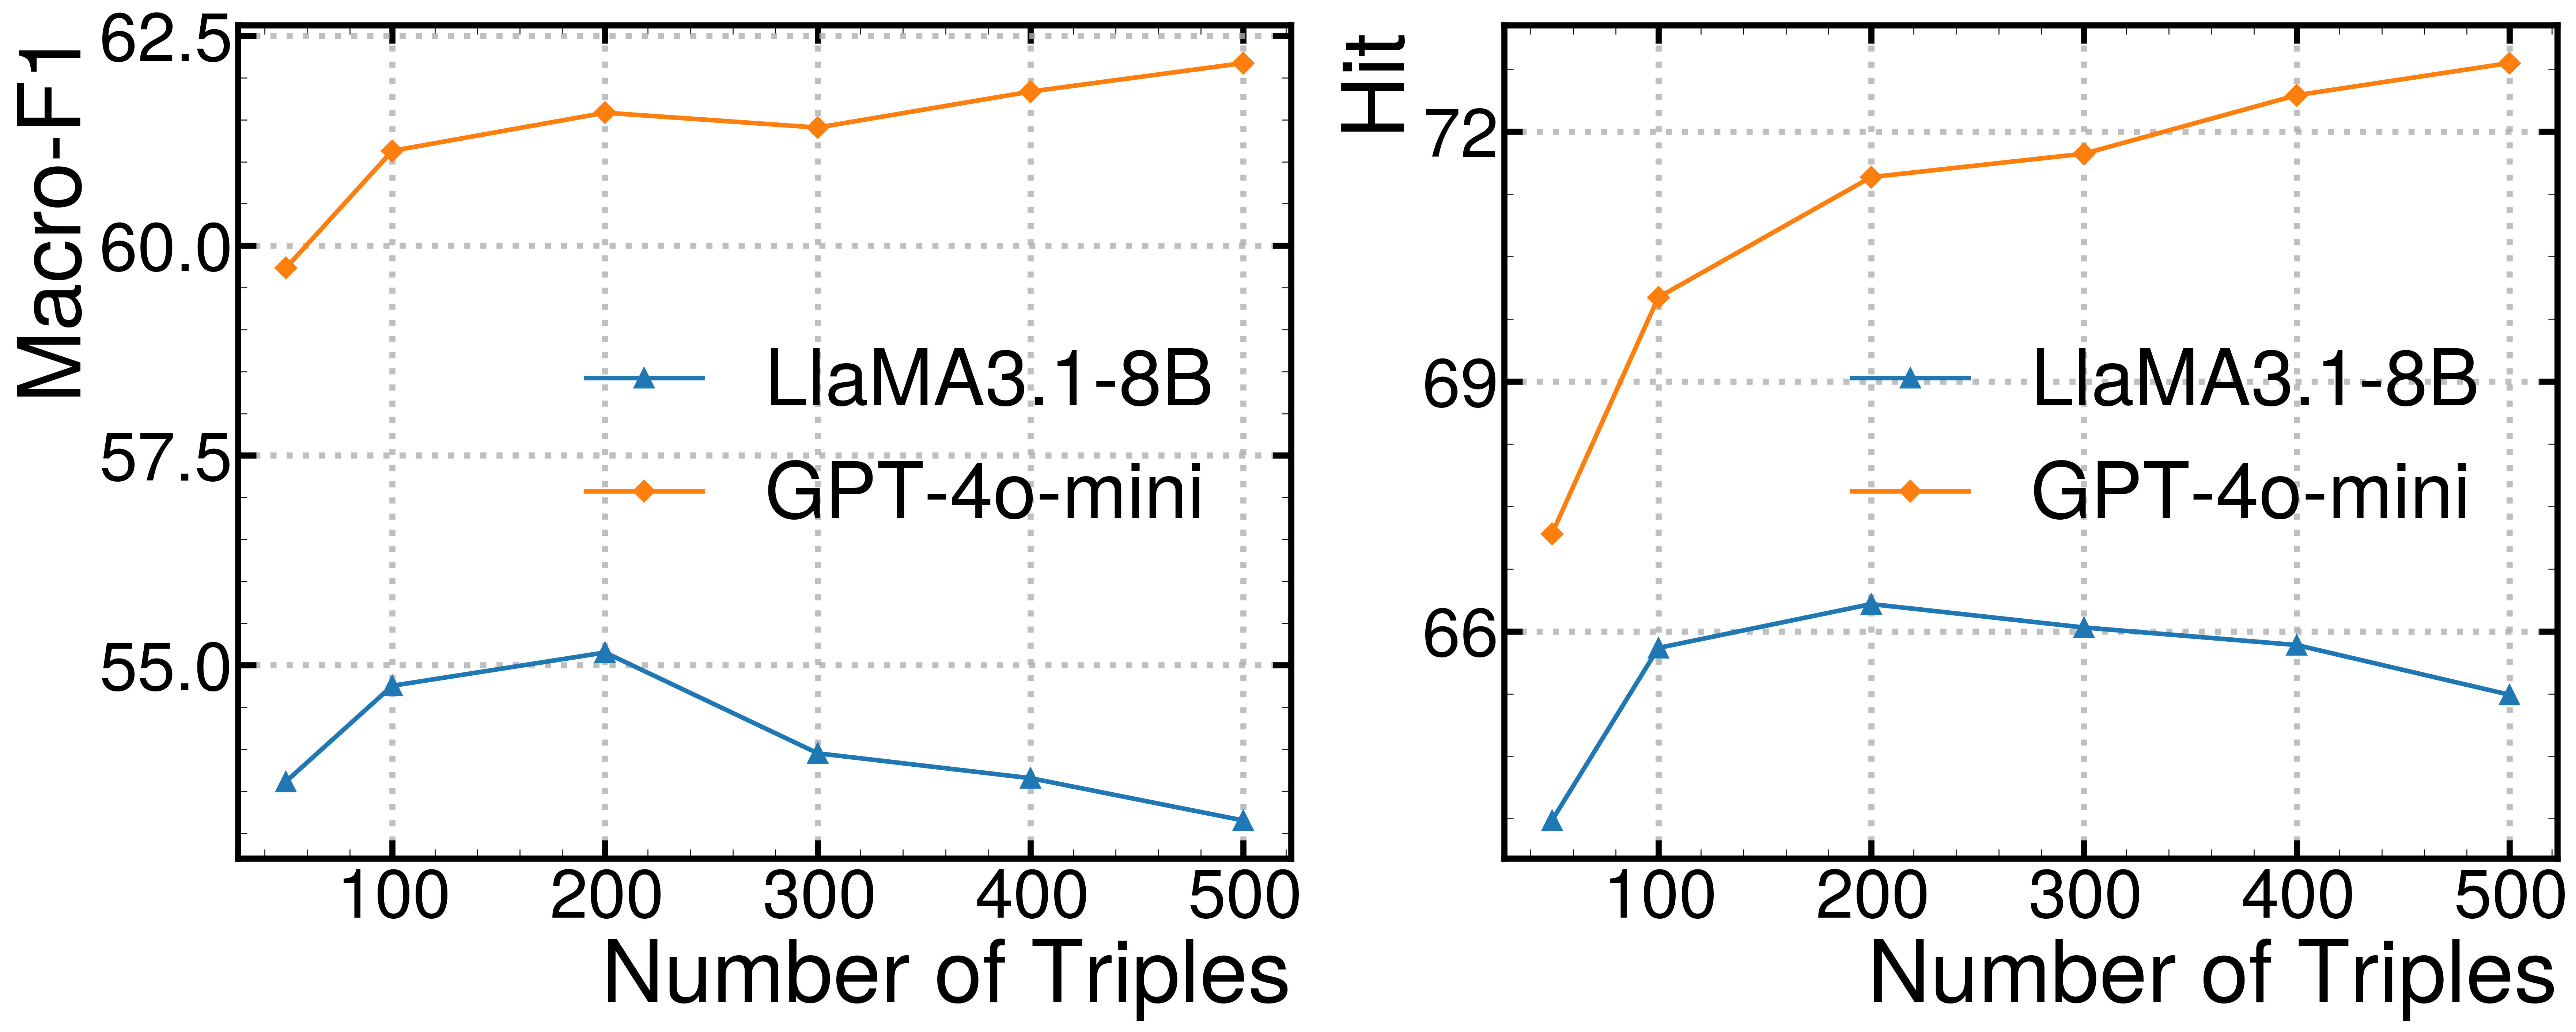
\includegraphics[trim={0cm 0.0cm 0.0cm 0cm}, clip,width=1.0\linewidth]{figs/numbers_cwq.png}
%         \caption{CWQ-sub}
%     \end{subfigure}
%     \vspace*{-2mm}
%     \caption{Ablation studies on the number of retrieved triples used in LLM reasoners.}
%     \label{fig:ablation_number}
%     \vspace{-4mm}
% \end{figure*}

\vspace{2mm}
\textbf{Experiment Settings.} We use the vllm~\citep{kwon2023efficient} framework for efficient LLM inference. For UniKGQA, KD-CoT, Retrieve-Rewrite-Answer, ToG, and EtD, we reference their published results due to various reproducibility difficulties. For StructGPT, we directly use their provided processed files to obtain results for WebQSP. For SR, we include their reported results for WebQSP and CWQ, and further evaluate it on WebQSP-sub as we could not run through SR's code on the two CWQ datasets. For the remaining baselines, we successfully reproduced their results and evaluated them on additional metrics and datasets, including WebQSP-sub and CWQ-sub. However, we do not include results for G-Retriever on CWQ as it required over 200 hours of computation on 2 NVIDIA RTX 6000 Ada GPUs. If not specified, the LLM reasoners in \proj use the top 100 retrieved triples; results using more triples are explicitly noted. All Llama models used are their instruction fine-tuned versions, i.e., Llama3.1-8B(70B)-Instruct. The used GPT models' versions are gpt-3.5-turbo-1106, gpt-4o-mini-2024-07-18, and gpt-4o-2024-08-06.
For all LLM reasoners used in \proj, both the temperature and the seed are set to 0 to ensure reproducibility.

\textbf{Overall Performance.} Tables~\ref{tab:QA_main} and~\ref{tab:QA_sub} present the results, where \proj achieves SOTA on WebQSP and WebQSP-sub. Even with 8B LLMs, our method surpasses previous SOTA approaches by $\leq 4\%$ in Macro-F1 and Hit metrics (excluding RoG-Joint due to test label leakage). With larger models like Llama3.1-70B-Instruct and GPT-4o, \proj achieves greater performance, showing $\leq 12\%$ improvement in Macro-F1 and $\leq 9\%$ in Hit.
On the more challenging CWQ and CWQ-sub datasets, which require more reasoning hops, \proj performs competitively with smaller 8B models. When paired with advanced LLMs like GPT-4o, \proj achieves results second only to ToG on CWQ. Notably, \proj requires only a single call to GPT-4o, whereas ToG requires 6-8 calls, which increases computational cost, and we were unable to reproduce ToG's performance using their published code. On CWQ-sub, \proj demonstrates gains of $\leq 9\%$ in Macro-F1 and $\leq 11\%$ in Hit, indicating that tasks with greater reasoning complexity benefit substantially from more powerful LLMs. Our method also excels in truth-grounded QA, with Score$_h$ consistently outperforming baselines by $\leq 12\%$, driven by our prompt design that encourages retrieval-grounded reasoning. See Appendix~\ref{appx:score} for further discussions.

Additionally, our framework generalizes well, with retrievers trained on one dataset performing effectively on others. Although moderate performance decay occurs due to domain shift, this can largely be mitigated by including more triples extracted by the retriever. Notably, the decay is generally minor on WebQSP and WebQSP-sub but more pronounced on CWQ and CWQ-sub, potentially due to greater label leakage from the WebQSP test set to the CWQ training set.

For efficiency, studies show that overall LLM latency is dominated by $\#$ LLM calls, followed by $\#$ output tokens and then $\#$ input tokens~\footnote{For LLMs like GPT-4 and Claude-3.5, an additional input token typically adds about $10^{-2}\times$ the latency of an extra output token and $10^{-4}\times$ that of an additional LLM call~\citep{vivek2024input}.}. \proj, despite potentially varying $\#$ input tokens, utilizes only one LLM call per question, whereas various baselines require multiple calls.

\textbf{Performance Breakdown \& Analysis.}
Table~\ref{tab:acc_hop} presents the performance breakdown by reasoning hops. 
Our method, even with an 8B LLM, shows significantly better results on multi-hop questions. This can be attributed to our design philosophy, which does not restrict the retrieved subgraph form and leverages unfine-tuned LLMs with ICL examples, fully unlocking their reasoning capabilities.
Interestingly, \proj shows relatively lower performance on some 1-hop questions in CWQ-sub. Cross-referencing with Table~\ref{tab:qa_breakdown}, which provides a detailed breakdown of whether the answers are truth-grounded, we find that previous methods may generate many correct answers that are not supported by the retrieved results.
Further investigation suggests this discrepancy may partly result from dataset leakage, giving tuning-based methods an advantage: In CWQ, over 60\% of test samples have answers that have appeared in the training set, making it easier for these methods to succeed without robust reasoning. Thus, future studies are needed to fully investigate the potential leakage.

\textbf{Performance with Different Retrievers.} 
To assess the impact of our retriever on the overall performance, we conducted extensive studies by replacing the retrieval results with those from baseline retrievers, while keeping all other settings constant (same prompts, same LLM reasoners).
Tables~\ref{tab:ablation_retriever_llama3} and~\ref{tab:ablation_retriever_4omini} show the results using Llama3.1 8B and GPT4o-mini as the LLM reasoners, respectively. For retrievers from Retrieve-Rewrite-Answer, StructGPT, G-Retriever, and RoG, we used all their retrieved triples, while for other cases, we kept 100 triples.
Clearly, pairing with our retriever yields significantly better performance on all metrics and datasets compared to using baseline retrievers, indicating that our superior results are largely due to the effectiveness of our improved retriever.

\label{para: reasoner_vary_k}
\textbf{Impact of Retrieval Size.} 
Irrelevant context can mislead LLMs~\citep{wu2024easily}, and retrieving more triples may not help. We conducted experiments (Fig.~\ref{fig:ablation_number}) by feeding Llama 3.1 8B and GPT-4o-mini different numbers of retrieved triples. The upper bound is defined such that if the answer entity is present in the retrieved results, it is considered a correct answer. The results show a significant performance decay in Llama 3.1 8B with more triples, while GPT-4o-mini performs even better with additional retrieved triples. This suggests that different LLMs have varying capacities for robust reasoning, and users should input proper numbers of retrieved results to match the capacity of the used LLM and the available computational budget. See Appendix~\ref{appx:score} for more results.

\textbf{Explainability.} By retrieving flexible, high-quality evidence subgraphs as context and exploiting the strong reasoning capabilities of pre-trained LLMs, \proj can natively provide effective explanations along with answer predictions. In contrast, explainable predictions with fine-tuned LLMs necessitate extra labeling efforts for preserving explainability~\citep{luo2024rog} or post hoc explainability approaches~\citep{krishna2023post}. To illustrate the explainability of our framework, we provide multiple examples of our reasoner's responses (see Appendix~\ref{appx:explain}).
